% Options for packages loaded elsewhere
\PassOptionsToPackage{unicode}{hyperref}
\PassOptionsToPackage{hyphens}{url}
%
\documentclass[
]{book}
\usepackage{lmodern}
\usepackage{amssymb,amsmath}
\usepackage{ifxetex,ifluatex}
\ifnum 0\ifxetex 1\fi\ifluatex 1\fi=0 % if pdftex
  \usepackage[T1]{fontenc}
  \usepackage[utf8]{inputenc}
  \usepackage{textcomp} % provide euro and other symbols
\else % if luatex or xetex
  \usepackage{unicode-math}
  \defaultfontfeatures{Scale=MatchLowercase}
  \defaultfontfeatures[\rmfamily]{Ligatures=TeX,Scale=1}
\fi
% Use upquote if available, for straight quotes in verbatim environments
\IfFileExists{upquote.sty}{\usepackage{upquote}}{}
\IfFileExists{microtype.sty}{% use microtype if available
  \usepackage[]{microtype}
  \UseMicrotypeSet[protrusion]{basicmath} % disable protrusion for tt fonts
}{}
\makeatletter
\@ifundefined{KOMAClassName}{% if non-KOMA class
  \IfFileExists{parskip.sty}{%
    \usepackage{parskip}
  }{% else
    \setlength{\parindent}{0pt}
    \setlength{\parskip}{6pt plus 2pt minus 1pt}}
}{% if KOMA class
  \KOMAoptions{parskip=half}}
\makeatother
\usepackage{xcolor}
\IfFileExists{xurl.sty}{\usepackage{xurl}}{} % add URL line breaks if available
\IfFileExists{bookmark.sty}{\usepackage{bookmark}}{\usepackage{hyperref}}
\hypersetup{
  pdftitle={Photochemistry and Photophysics Workshops},
  pdfauthor={Fiona Dickinson},
  hidelinks,
  pdfcreator={LaTeX via pandoc}}
\urlstyle{same} % disable monospaced font for URLs
\usepackage{longtable,booktabs}
% Correct order of tables after \paragraph or \subparagraph
\usepackage{etoolbox}
\makeatletter
\patchcmd\longtable{\par}{\if@noskipsec\mbox{}\fi\par}{}{}
\makeatother
% Allow footnotes in longtable head/foot
\IfFileExists{footnotehyper.sty}{\usepackage{footnotehyper}}{\usepackage{footnote}}
\makesavenoteenv{longtable}
\usepackage{graphicx,grffile}
\makeatletter
\def\maxwidth{\ifdim\Gin@nat@width>\linewidth\linewidth\else\Gin@nat@width\fi}
\def\maxheight{\ifdim\Gin@nat@height>\textheight\textheight\else\Gin@nat@height\fi}
\makeatother
% Scale images if necessary, so that they will not overflow the page
% margins by default, and it is still possible to overwrite the defaults
% using explicit options in \includegraphics[width, height, ...]{}
\setkeys{Gin}{width=\maxwidth,height=\maxheight,keepaspectratio}
% Set default figure placement to htbp
\makeatletter
\def\fps@figure{htbp}
\makeatother
\setlength{\emergencystretch}{3em} % prevent overfull lines
\providecommand{\tightlist}{%
  \setlength{\itemsep}{0pt}\setlength{\parskip}{0pt}}
\setcounter{secnumdepth}{5}
\usepackage{booktabs}
\usepackage{amsthm}
\makeatletter
\def\thm@space@setup{%
  \thm@preskip=8pt plus 2pt minus 4pt
  \thm@postskip=\thm@preskip
}
\makeatother
\usepackage[]{natbib}
\bibliographystyle{apalike}

\title{Photochemistry and Photophysics Workshops}
\author{Fiona Dickinson}
\date{2020-10-15}

\begin{document}
\maketitle

{
\setcounter{tocdepth}{1}
\tableofcontents
}
\hypertarget{welcome}{%
\chapter*{Welcome}\label{welcome}}
\addcontentsline{toc}{chapter}{Welcome}

The notes have been prepared in a package called BookDown for RStudio so that the equations are accessible to screen readers. However, by providing the notes as a .html webpage I can also embed short videos to further describe some of the topics. Further you can download the questions (and later the answers, top left of the screen) in a format that suits you (either pdf or epub) to view offline, or change the way this document appears for ease of reading.

\hypertarget{workshops-for-photochemistry-photophysics}{%
\section*{Workshops for Photochemistry \& Photophysics}\label{workshops-for-photochemistry-photophysics}}
\addcontentsline{toc}{section}{Workshops for Photochemistry \& Photophysics}

The course will use a question first approach and we will learn the material by answering the questions. The questions will are shared here in an accessible format, and this page will be updated weekly.

This is the answers for workshop questions, the answers have been prepared from collaborative problem solving from the CH30129 class of 2020-21.

\hypertarget{version-history}{%
\section*{Version history}\label{version-history}}
\addcontentsline{toc}{section}{Version history}

Week three answers finished 151020
Week two answers finished 061020
Week one answer for final question finished 051020
Week one answers finished 300920
The initial commit of this book is dated 29th September 2020.

\hypertarget{ch:Workshop1}{%
\chapter{Workshop Answers for Week 1}\label{ch:Workshop1}}

\hypertarget{sec:BeerLambert}{%
\section{Short mathematical question - Beer Lambert law}\label{sec:BeerLambert}}

- \emph{How far can monochromatic 489 nm light travel through a 0.100 M solution of fluorescein with an extinction coefficient at 489 nm of 92000 M\textsuperscript{−1} cm\textsuperscript{−1} before 90 \% of it is absorbed?}

If 90\% of the incident light is being absorbed then 10\% of the light is transmitted\ldots{}

The Beer-Lambert law is (Equation \eqref{eq:BeerLambert}):

\begin{equation}
\log{\frac{I}{I_0}}=-\varepsilon c l
\label{eq:BeerLambert}
\end{equation}

rearranging this:

\begin{equation*}
l = \frac{\log{\frac{I_0}{I}}}{\varepsilon c}
\end{equation*}

\begin{equation*}
l = \frac{\log{\frac{100 \%}{10 \%}}}{92000 \textrm{ M}^{-1} \textrm{ cm}^{-1} \times 0.100 \textrm{ M}}
\end{equation*}

\begin{equation*}
l = \frac{1}{9200000 \textrm{ M}^{-1} \textrm{ m}^{-1} \times 0.100 \textrm{ M}}
\end{equation*}

\begin{equation*}
l = 1.0 \textrm{ μm}
\end{equation*}

\hypertarget{sec:MolarExtinction}{%
\section{Short conceptual question - molar extinction coefficient}\label{sec:MolarExtinction}}

\emph{- Modify the molecule in figure \ref{fig:bpy} to increase the molar extinction coefficient (do not worry about what may happen to wavelength).}

\begin{figure}

{\centering 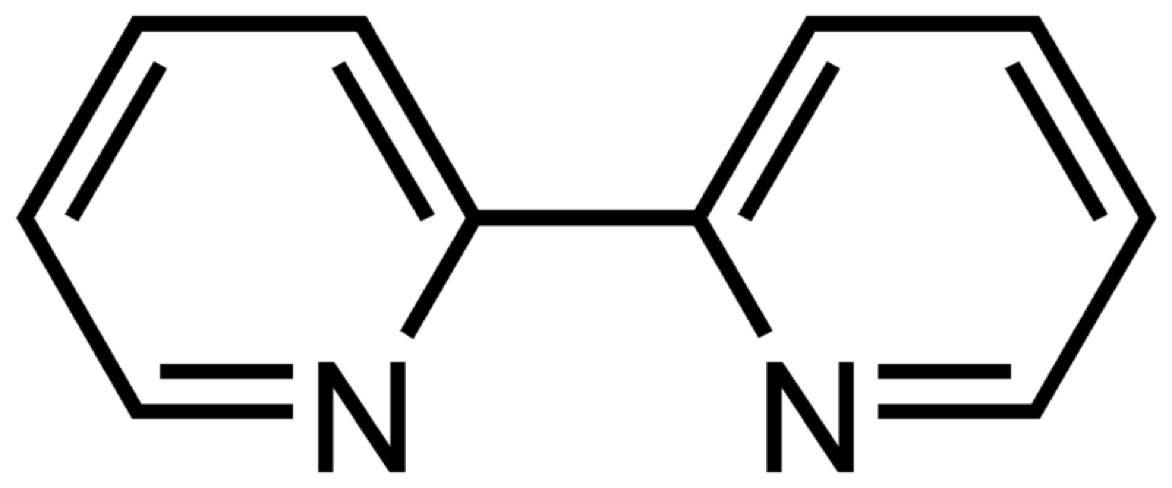
\includegraphics[width=0.3\linewidth]{images/bpy} 

}

\caption{The structure of bipyridine (also known as bpy).}\label{fig:bpy}
\end{figure}

If a molecule is rigid the difference between the ground and excited state structure is smaller and this usually leads to a higher molar extinction coefficient, so any structural changes which increase this rigidity will likely lead to a higher molar extinction coefficient.

\begin{figure}

{\centering 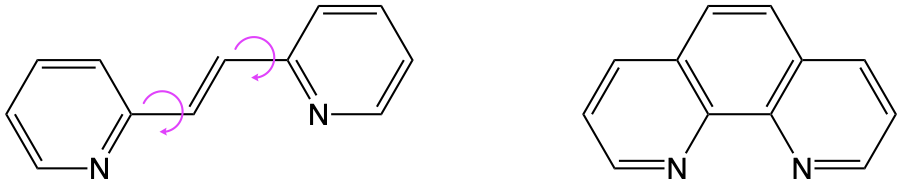
\includegraphics[width=1\linewidth]{images/structurealts} 

}

\caption{Two possible modifications of bpy, the stilbene derivative on teh left has a very different ground and excited state structure due to the possible rotations around the two conjucated single bonds, the phenantroline modificaiton on the right does not allow much deviation in structure and so the excited state is only bent as the bond order is reduced leading to a larger overlap integral.}\label{fig:bpyalts}
\end{figure}

Excitation of an electron from a bonding or non-bonding orbital into an anti-bonding orbital reduces the bond order, and will `kink' aromatic systems.

\hypertarget{sec:intensity}{%
\section{Short conceptual question - intensity of colour}\label{sec:intensity}}

\emph{- What factors influence the `intensity of colour' of the following solutions?}

\begin{figure}

{\centering 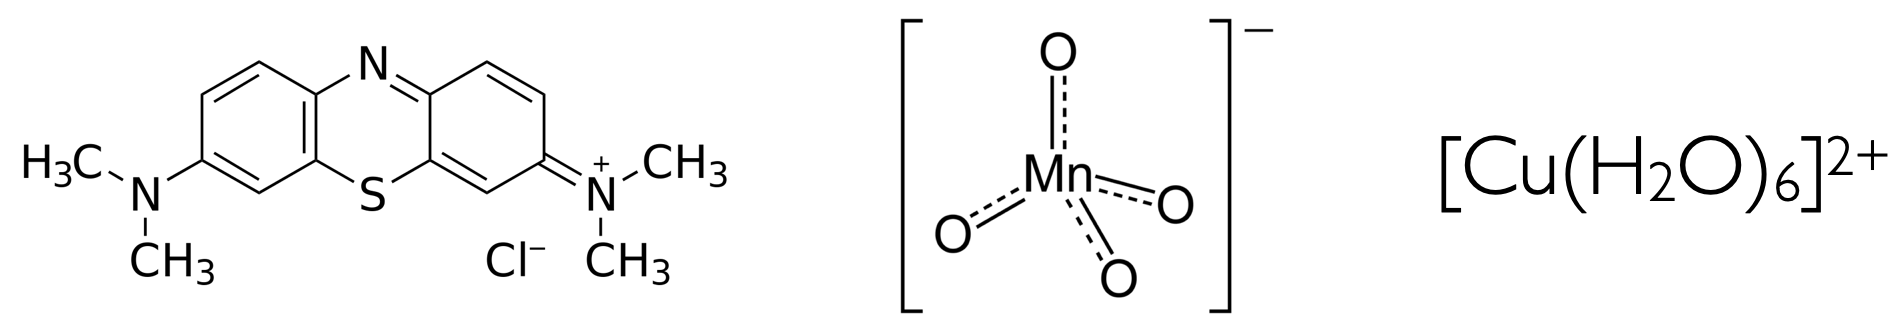
\includegraphics[width=0.7\linewidth]{images/molarextquestion} 

}

\caption{The structures of the organic dye methylene blue (left), potassium permanganate (centre) and copper hexa-aqua (right).}\label{fig:molarextstructures}
\end{figure}

\begin{figure}

{\centering 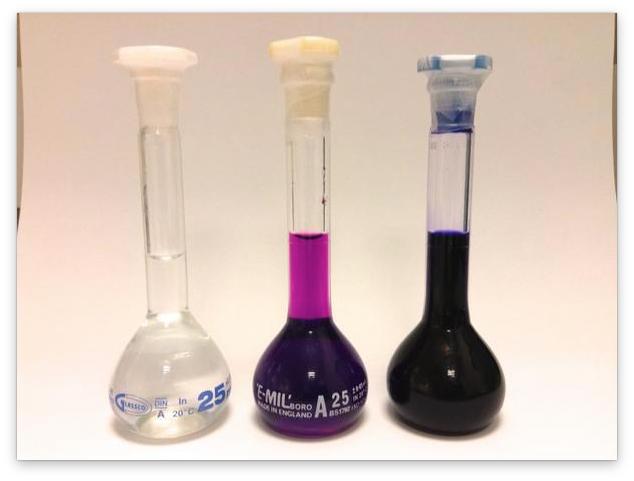
\includegraphics[width=0.7\linewidth]{images/Molar_extinction_coefficients} 

}

\caption{1 mM solutions of the organic dye methylene blue (right), potassium permanganate (centre) and copper (hexa-aqua) sulfate (left).}\label{fig:molarextsolutions}
\end{figure}

CuSO\textsubscript{4} in solution forms the hexa aqua complex listed in figure \ref{fig:molarextstructures}. This is a centrosymmetric molecule which therefore runs foul of the Laporte selection rule which says that ``allowed transitions in centrosymmetric molecules must involve a change in parity''. So either g → u or u → g are allowed, and g → g and u → u are forbidden.

You will not be expected to work out symetry types for orbitals but can `back justify' to explain with this.

These symmetry labels appear on the energy level diagram for CU\textsuperscript{2+} (figure \ref{fig:Cu}).

\begin{figure}

{\centering 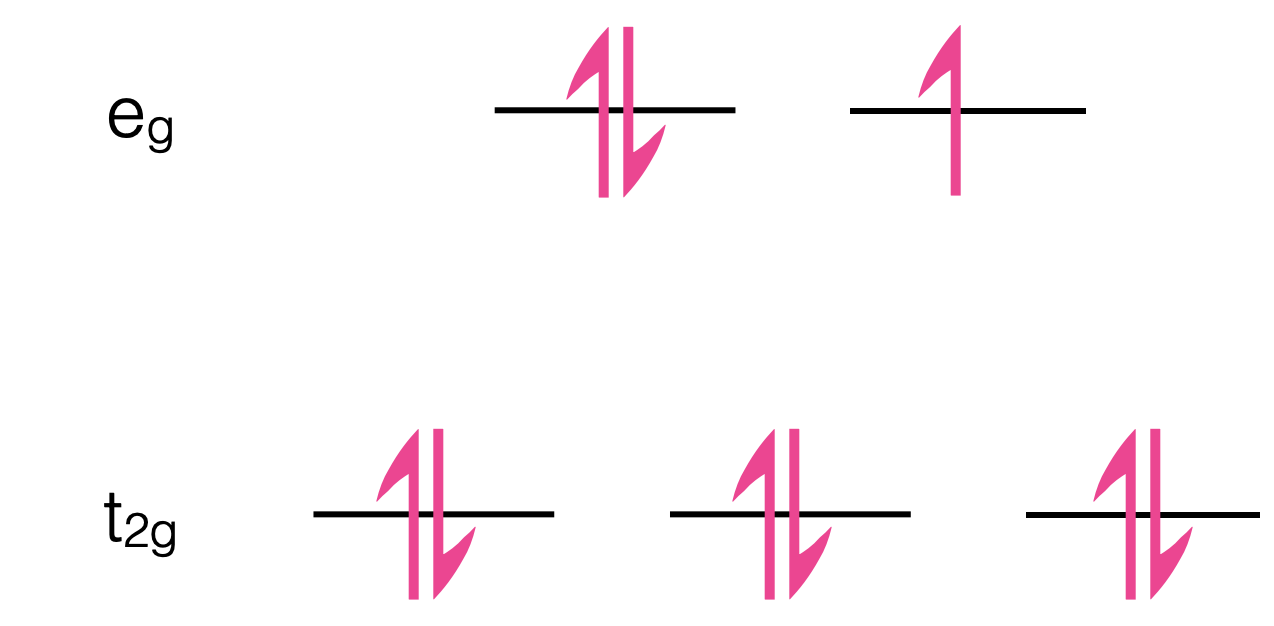
\includegraphics[width=0.4\linewidth]{images/CuIIenergylevels} 

}

\caption{The splitting of the d-orbitals in octahedral Cu2+, the transition is between the HOMO t2g level and the PUMO eg level. The subscript g on each of these orbitals is a symmetry label indicating there is no change or parity and so the transition is Laporte forbidden.}\label{fig:Cu}
\end{figure}

Both of the split energy levels are gerade (g) and so there is no change of parity for the transition from t\textsubscript{2g} to e\textsubscript{g}, therefore the transition is selection rule forbidden and has a low molar extinction coefficient. The `breaking of symmetry' by possible rotamers of the water ligands mean this value is higher than for the gas phase atomic molar absorption coefficient. The maximum molar extinction coefficient of copper sulfate solutions is around 20 M\textsuperscript{-1} cm\textsuperscript{-1}.

The permanganate (MnO\textsubscript{4}\textsuperscript{-}) is a ligand to metal charge transfer transition, since excitation of an electron effectively moves an electron from one of the oxygen ligands to the manganese `empty' metal centre there is no limitation from the spin selection rule and the complex is not subject to the Laporte selection rule. This leads to moderate to `high' molar extinction coefficients. The maximum molar extinction coefficient of potassium permanganate solutions is around 1800 M\textsuperscript{-1} cm\textsuperscript{-1}.

The final molecule is the synthetic dye methylene blue, this is not centrosymmetric and so is not subject to the Laporte selectrion rule, further the structure with fused aromatic rings and a large amount of conjugation is fairly rigid and so there is a large overlap of the wavefunctions of the ground and excited state. The maximum molar extinction coefficient of methylene blue solutions is around 75000 M\textsuperscript{-1} cm\textsuperscript{-1}.

\hypertarget{sec:linewidth}{%
\section{Short conceptual question - line width}\label{sec:linewidth}}

- \emph{Why are some spectra very broad (figure \ref{fig:molecular}), whereas others have sharp peaks (figure \ref{fig:atomic})?}

\emph{You will need to look at the x-scale to truley note the difference in the width of these emission spectra.}

\begin{figure}

{\centering 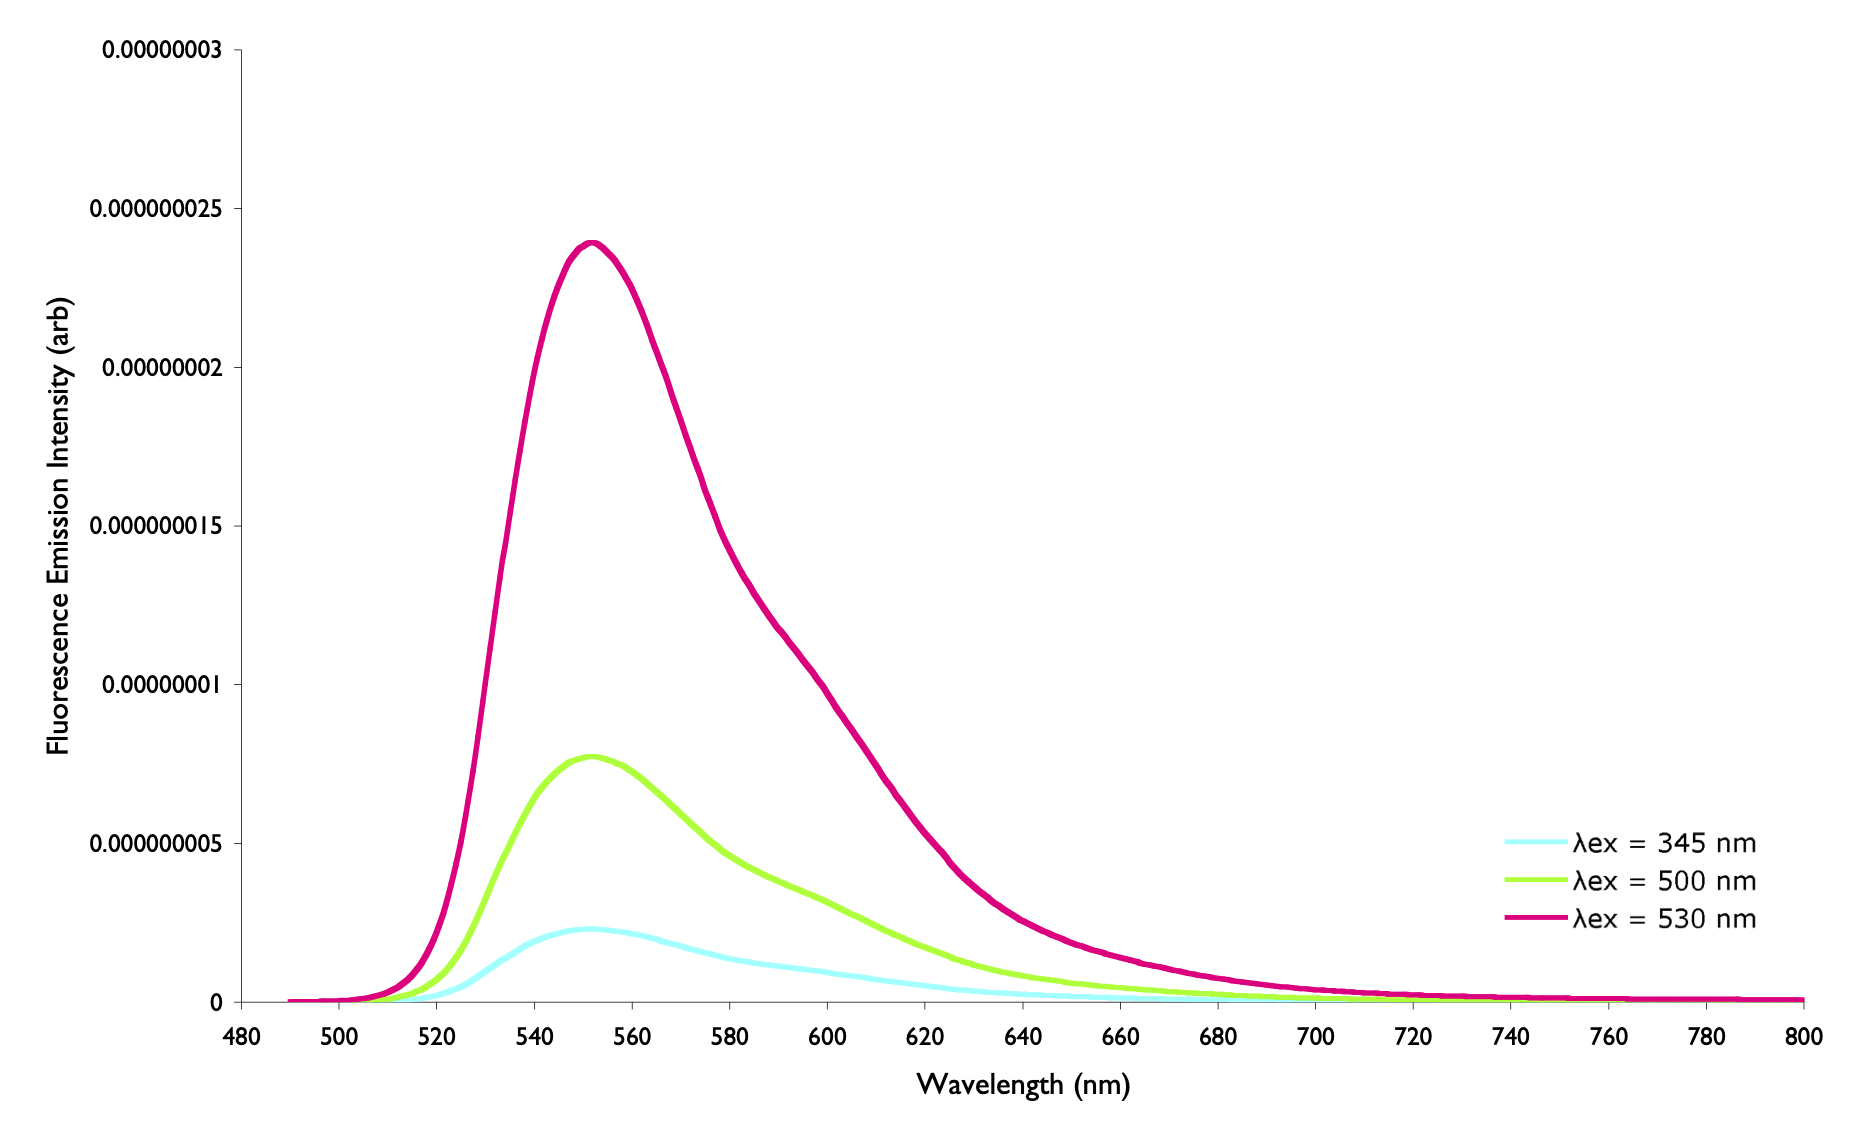
\includegraphics[width=0.7\linewidth]{images/rhodamine6G} 

}

\caption{The fluorescence emission spectrum of rhodamine 6G in methanol}\label{fig:molecular}
\end{figure}

\begin{figure}

{\centering 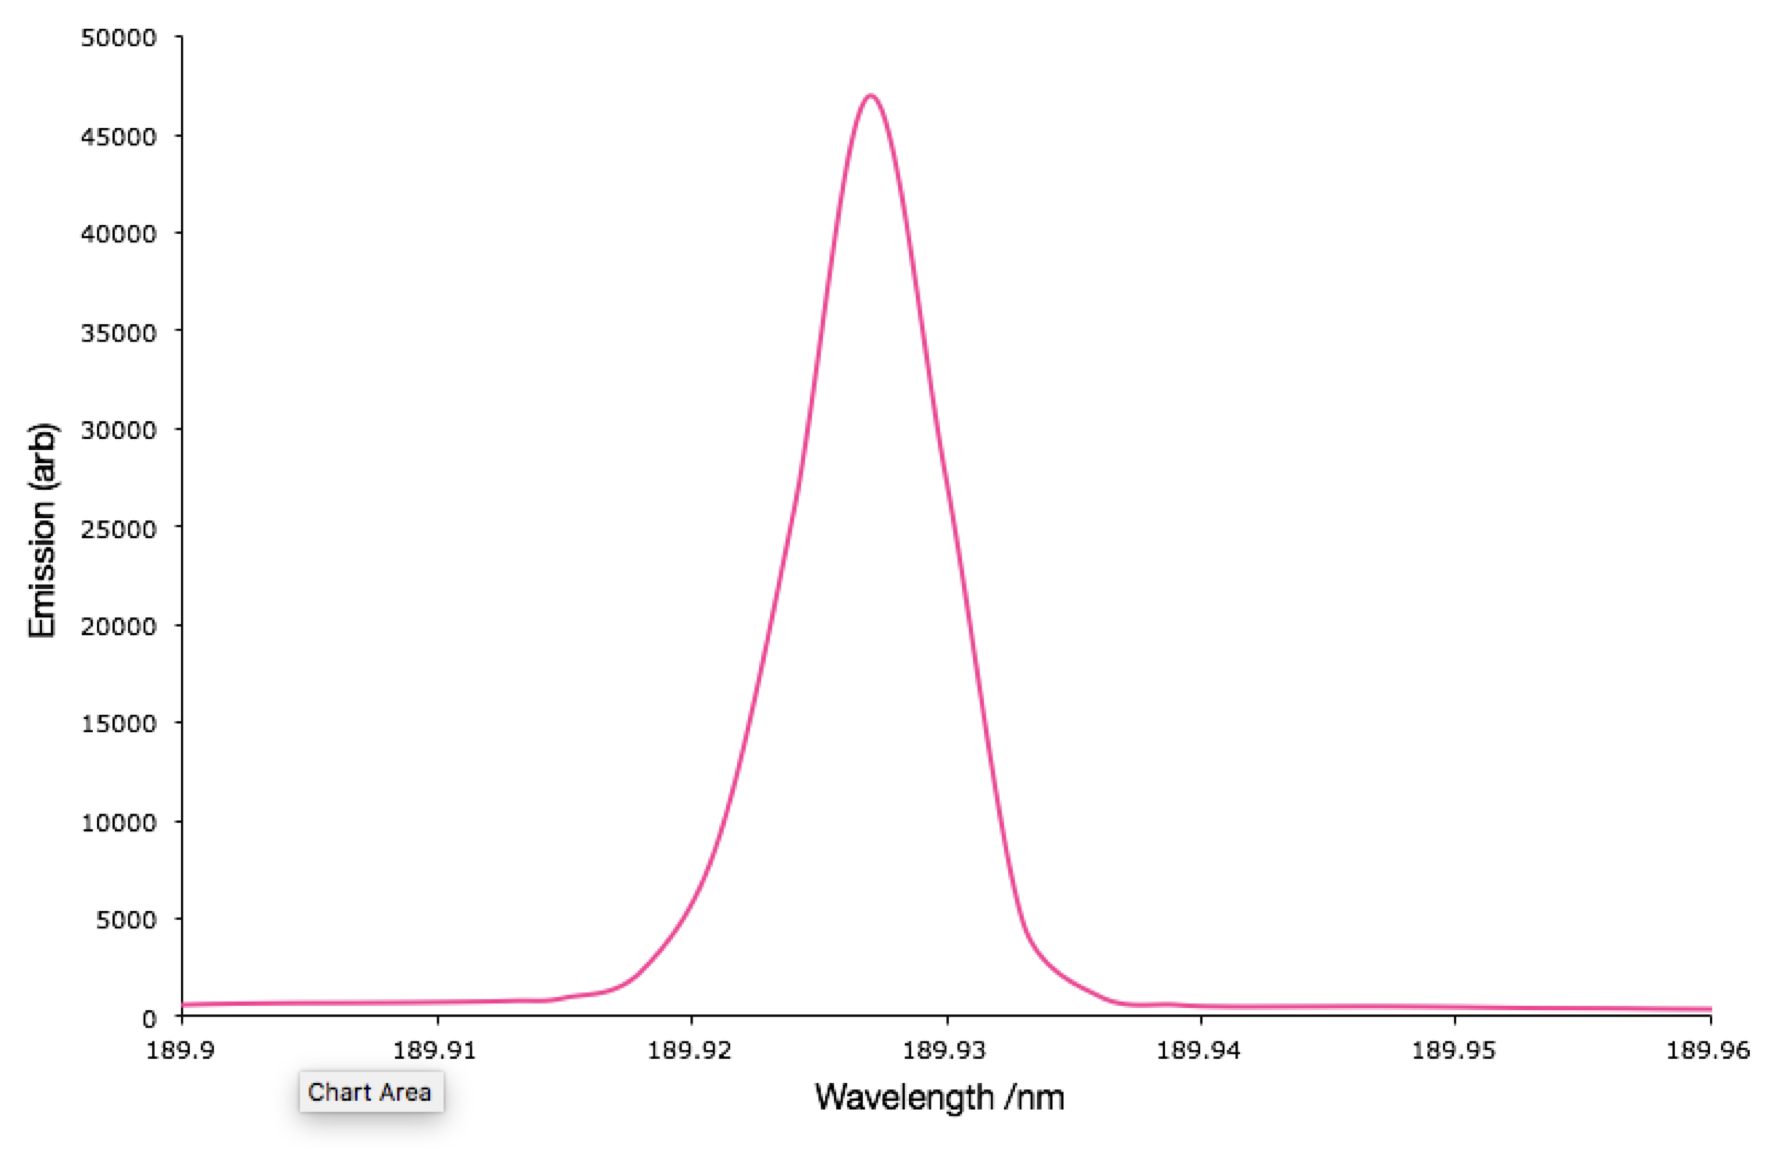
\includegraphics[width=0.7\linewidth]{images/atomic_emission_spectrum} 

}

\caption{The emission spectrum of Sn(II) from ICP-OES}\label{fig:atomic}
\end{figure}

We are looking at two very different spectra here, first off we have an atomic transition and a molecular transition. Secondly one is solvated, the other in the gas (or more acurately plasma) phase. Both of these factors are important\ldots{}

When we have a transition for either absorption or emission then on an atomic level those energy levels are incredibly well defined, this leads to the energy required to promote an electron between these levels to be equally well defined.

As soon as we solvate this the energy of the occupied (HOMO) is softened as intermolecular interactions will stabilise this level to different amounts, solvation may also allow previously absolutely parity forbidden processes to occur.

The molecular spectrum is much broader because each of the possible rotamers, vibratamers and isomers has a slightly different energy, the myriad possible energies are expanded still by solvation and tempeature effects. The more possible structural isomers and rotamers the `softer' any defining features in the spectrum. For example if we compare the rhodamine spectum (figure \ref{fig:molecular}) to that of antracene (figure \ref{fig:anthracene}) we can see that there is more `fine structure' in the anthracene spectrum, this is because of the smaller possible number of structural variations, there are no possible rotamers and so transitions are more defined.

\begin{figure}

{\centering 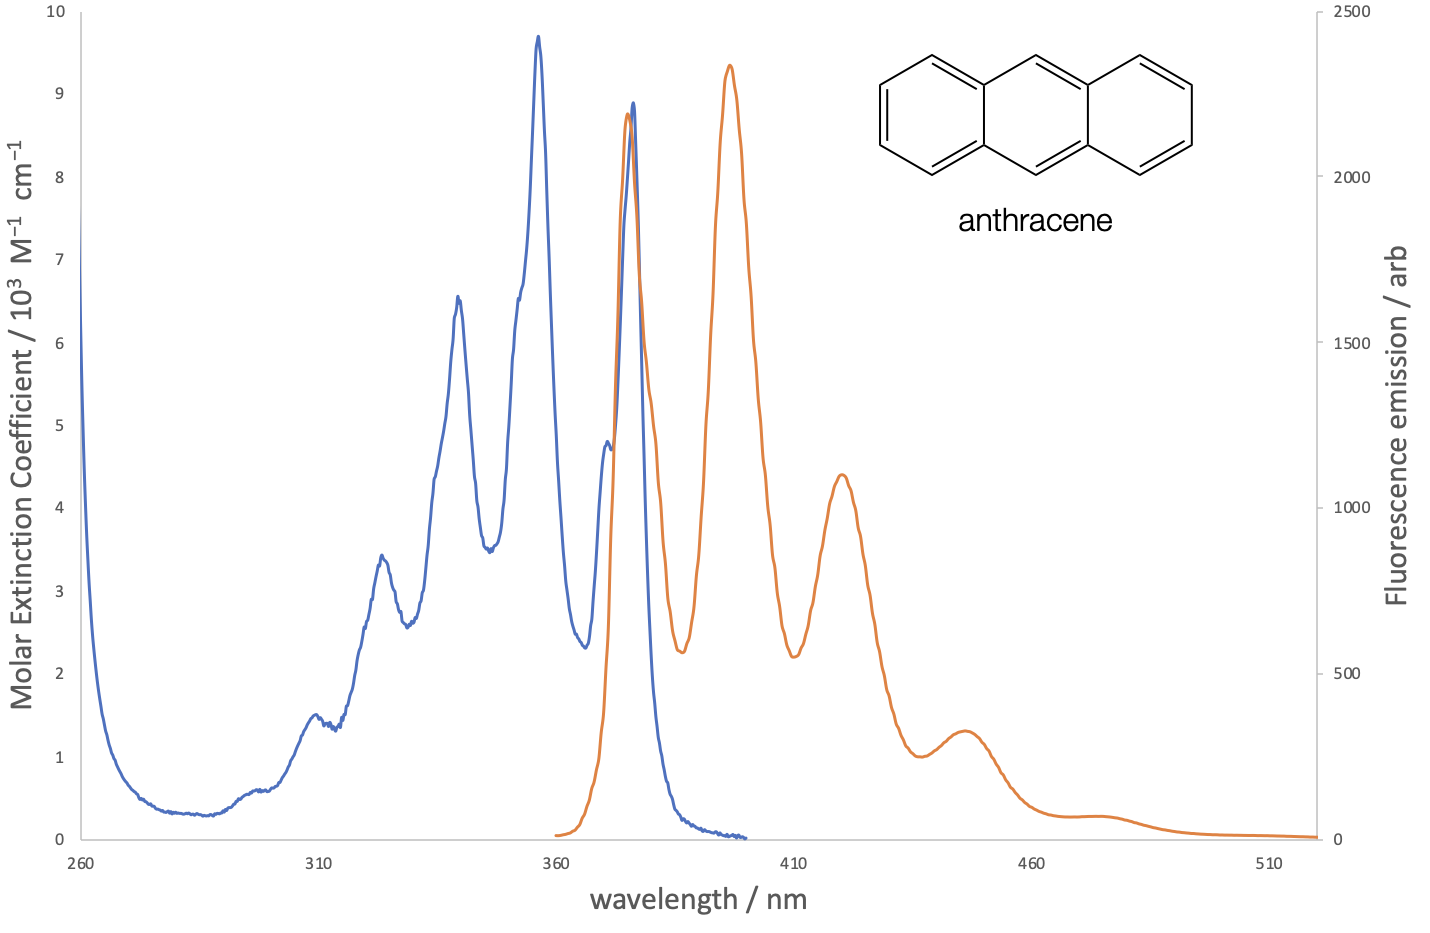
\includegraphics[width=0.7\linewidth]{images/anthracene} 

}

\caption{The absorption and emission spectra of anthracene indicating fine structure in the spectrum}\label{fig:anthracene}
\end{figure}

\hypertarget{sec:solvationabs}{%
\section{Short conceptual question - the effect of solvation on absorbance}\label{sec:solvationabs}}

\begin{figure}

{\centering 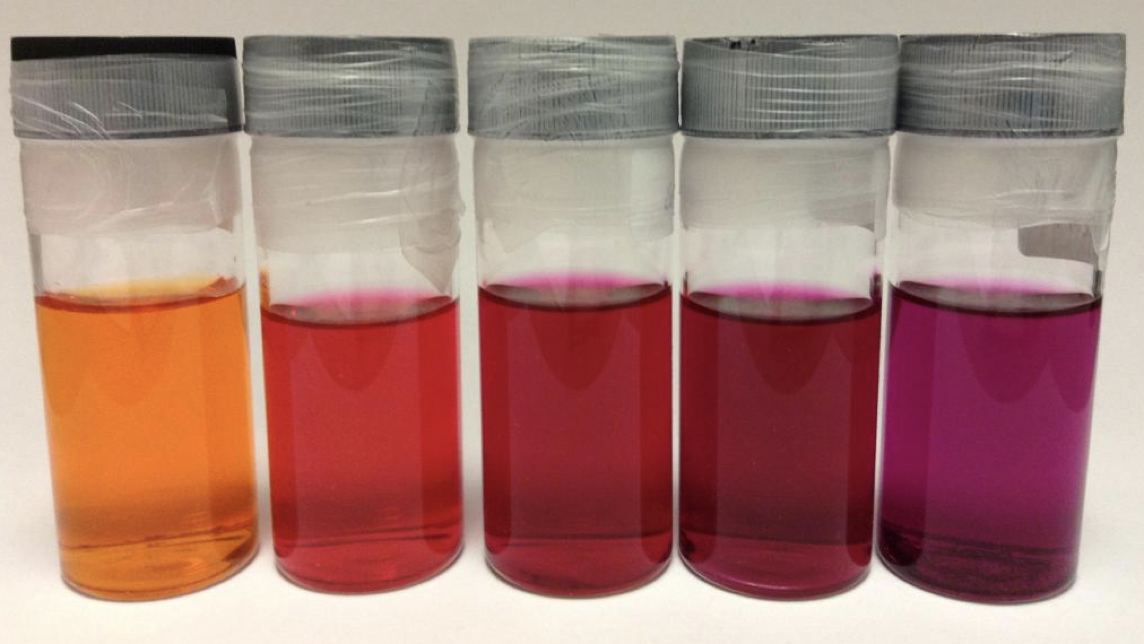
\includegraphics[width=0.7\linewidth]{images/ethidium} 

}

\caption{Ethidium bromide dissolved in from right; water(orange), methanol, ethanol, propanol and butanol(purple)}\label{fig:ethidium}
\end{figure}

- \emph{Why does the observed colour of ethidium bromide depend upon the solvent (figure \ref{fig:ethidium}))?}

\emph{Think about the effect of solvation on the energy levels and why those energy levels matter! Remember that if light is transmitted through a solution that is the colour we observe\ldots{}}

This is in essence answering the same question as in question \ref{sec:linewidth}, solvation affects the energy levels of occupied orbitals.WIthout going into any more detail than essential the different solvents stabilise the HOMO of ethidium bromide different amounts - this is likely due to different hydrogen bonding of the alchols. The more stabilised the ground state the bigger the energy gap leading to a blue shift in the absorption spectra. The orange solution is absorbing blue light (λ\textsubscript{max} = 480 nm) and the purple solution absorbing orange (λ\textsubscript{max} = 550 nm) indicating the energy gap of the aquous solution is larger and therefore the solvent stabilisation is biggest.

It is worth noting that the energy of `empty' orbitals is unaffected and so the energy of the LUMO is unchanged (figure \ref{fig:solvato}).

\begin{figure}

{\centering 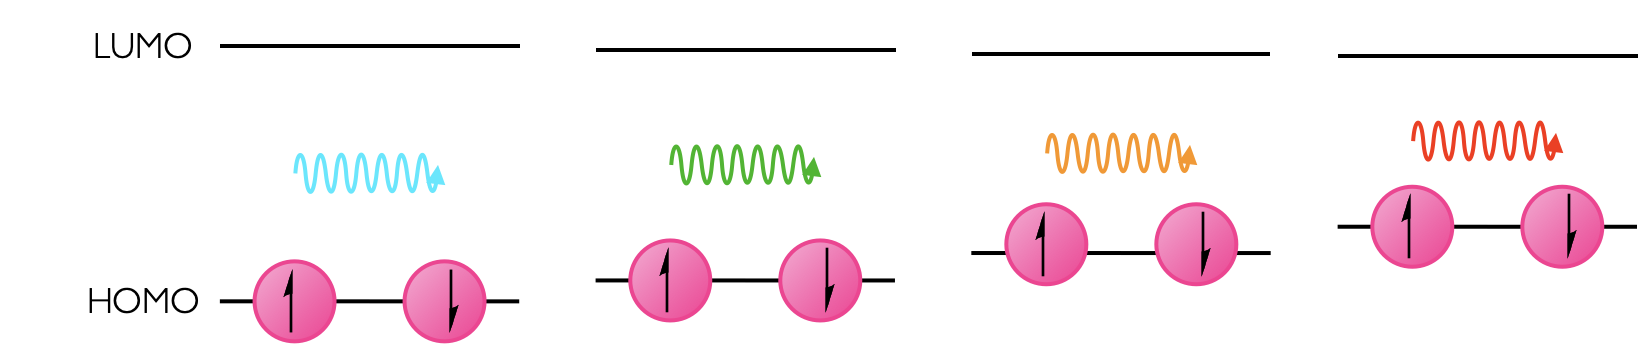
\includegraphics[width=0.7\linewidth]{images/solvatochromism} 

}

\caption{Solvation effects the energy level of the HOMO, but the unoccupied LUMO always has the same energy, conseqently in different solvents the energy gap varies.}\label{fig:solvato}
\end{figure}

\hypertarget{sec:Azobenzene}{%
\section{Extended question - Azobenzene}\label{sec:Azobenzene}}

\emph{Azobenzene undergoes the following cis-trans isomerisation, the isomerisation occurs in the ps timescale.}

\begin{figure}

{\centering 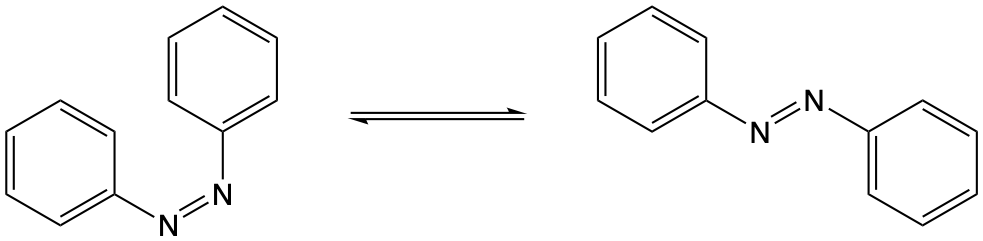
\includegraphics[width=0.7\linewidth]{images/cistransazobenzene} 

}

\caption{The cis-trans isomerisation of azobenzene}\label{fig:cistransazobenzene}
\end{figure}

- \emph{Why would you expect the absorption spectrum of each isomer to be different?}

Trans azobenzene is centrosymmetric and so is subject to the Laporte selection rule, cis azobenzene is non-centrosymmetric and so it is not parity forbidden. Consequently the HOMO-LUMO transition which is allowed for the cis is forbidden for the trans and so the absorbance spectra is different.

- \emph{Suggest why the trans conformation is more stable than the cis isomer.}

Steric hinderance will mean that the cis-isomer is not planar, if it isn't planar it isn't fully conjugated, and if it isn't fully conjugated it isn't as stable. There is no steric hinderance in the trans isomer.

- \emph{Use the following data to predict the proportion of each isomer under 360 nm excitation.}

\emph{Table: \label{tab:azobenzeneabs} The molar extinction coefficient of the two isomers of azobenzene.}

\begin{longtable}[]{@{}lll@{}}
\toprule
& ε\textsubscript{360} / M\textsuperscript{−1} cm\textsuperscript{−1} & ε\textsubscript{460} / M\textsuperscript{−1} cm\textsuperscript{−1}\tabularnewline
\midrule
\endhead
trans-azobenzene & 22000 & 4500\tabularnewline
cis-azobenzene & 2100 & 5500\tabularnewline
\bottomrule
\end{longtable}

For the photostationary state the absorbance of the two isomers will be the same.

The excited state for both molecules will be the same, and the probability of the excited state decaying into any given isomer is the same.

So if \(A =\varepsilon cl\) and \(A_{trans}=A_{cis}\) then at 360 nm:

\begin{equation*}
\varepsilon_{trans} c_{trans} = \varepsilon_{cis} c_{cis}
\end{equation*}

\(c_{trans}= 0.095 c_{cis}\)

- \emph{Would there be more or less trans azobenzene at 460 nm? Justify your answer.}

There would be more trans at the photostationary state when excited at 460 nm, this is because the relative ration of molar extinction coefficients favors formation of more of the trans isomer.

- \emph{It has been suggested the 360 nm absorption is an S\textsubscript{0} → S\textsubscript{2} absorption, and the 460 nm band is an S\textsubscript{0} → S\textsubscript{1} absorption. Suggest which energy levels are involved for each of the two transitions and compare it to stilbene which has a similar structure, but the cis and trans absorptions are 280 \& 295 nm respectively.}

\begin{figure}

{\centering 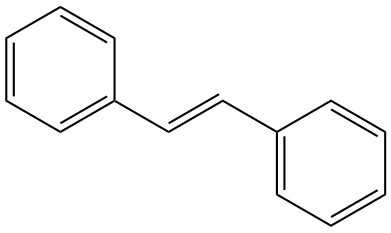
\includegraphics[width=0.3\linewidth]{images/stilbene} 

}

\caption{The  structure of stilbene}\label{fig:stilbene}
\end{figure}

Azobenzene has \(n\), \(\pi\) and \(\pi^*\) orbitals whereas stilbene only has \(\pi\) and \(\pi^*\) orbitals. Given the different orbital types available in azobenzene the expectation that the transitions will have a wider energy spacing than in stilbene where we just have the bonding and antibonding \(pi\) set, and so we would expect these energy levels to be more closely spaced.

I'm leaving you hanging on this one we will discuss it again next week.

\hypertarget{ch:Workshop2}{%
\chapter{Workshop Answers for Week 2}\label{ch:Workshop2}}

\hypertarget{sec:YieldLifetime}{%
\section{Short mathematical question - Quantum Yield and lifetime}\label{sec:YieldLifetime}}

\emph{The quantum yield and lifetime of a dye were measured to be 0.43 \& 2.6 ns respectively. What is the natural lifetime?}

The fluorescence quantum yield (equation \eqref{eq:lifetimefluor} and fluorescence lifetime (equation \eqref{eq:lifetimefluor}) are related to the rate constants for the different decay processes.

\begin{equation}
\phi_f = \frac{k_f^0}{k_f^0+k_{ic}+ k_{ST}+k_{\textrm{other}}}
\label{eq:QYfluor}
\end{equation}

\begin{equation}
\tau_f = \frac{1}{k_f^0+k_{ic}+ k_{ST}+k_{\textrm{other}}}
\label{eq:lifetimefluor}
\end{equation}

The natural lifetime is the lifetime when the only decay pathway is fluorescence emission (equation \eqref{eq:natural}).

\begin{equation}
\tau_f^0 = \frac{1}{k_f^0}
\label{eq:natural}
\end{equation}

Combining equations \eqref{eq:lifetimefluor} and \eqref{eq:lifetimefluor}:

\begin{equation*}
\frac{\tau_f}{\phi_f}=\frac{\frac{1}{k_f^0+k_{ic}+ k_{ST}+k_{\textrm{other}}}}{\frac{k_f^0}{k_f^0+k_{ic}+ k_{ST}+k_{\textrm{other}}}}=\frac{1}{k_f^0}=\tau_f^0
\end{equation*}

Consequently \(\tau_f^0 = \frac{\tau_f}{\phi_f}=\frac{2.6}{0.43}= 6.0\) ns

\hypertarget{sec:otherprocesses}{%
\section{Short conceptual question - Effect of other processes}\label{sec:otherprocesses}}

\emph{For a given value of τ\textsubscript{0} what happens to the lifetime and quantum yield as k\textsubscript{IC} and k\textsubscript{ISC} increases?}

If \(k_f^0\) is fixed (which it is for a given chromophore) then as we adjust the other rate constants in equation \eqref{eq:lifetimefluor} the emission lifetime (the time it takes for the intensity to reduce to 1/e of the initial intensity) decreases, as shown in figure \ref{fig:rateslifetime}.

\begin{figure}

{\centering 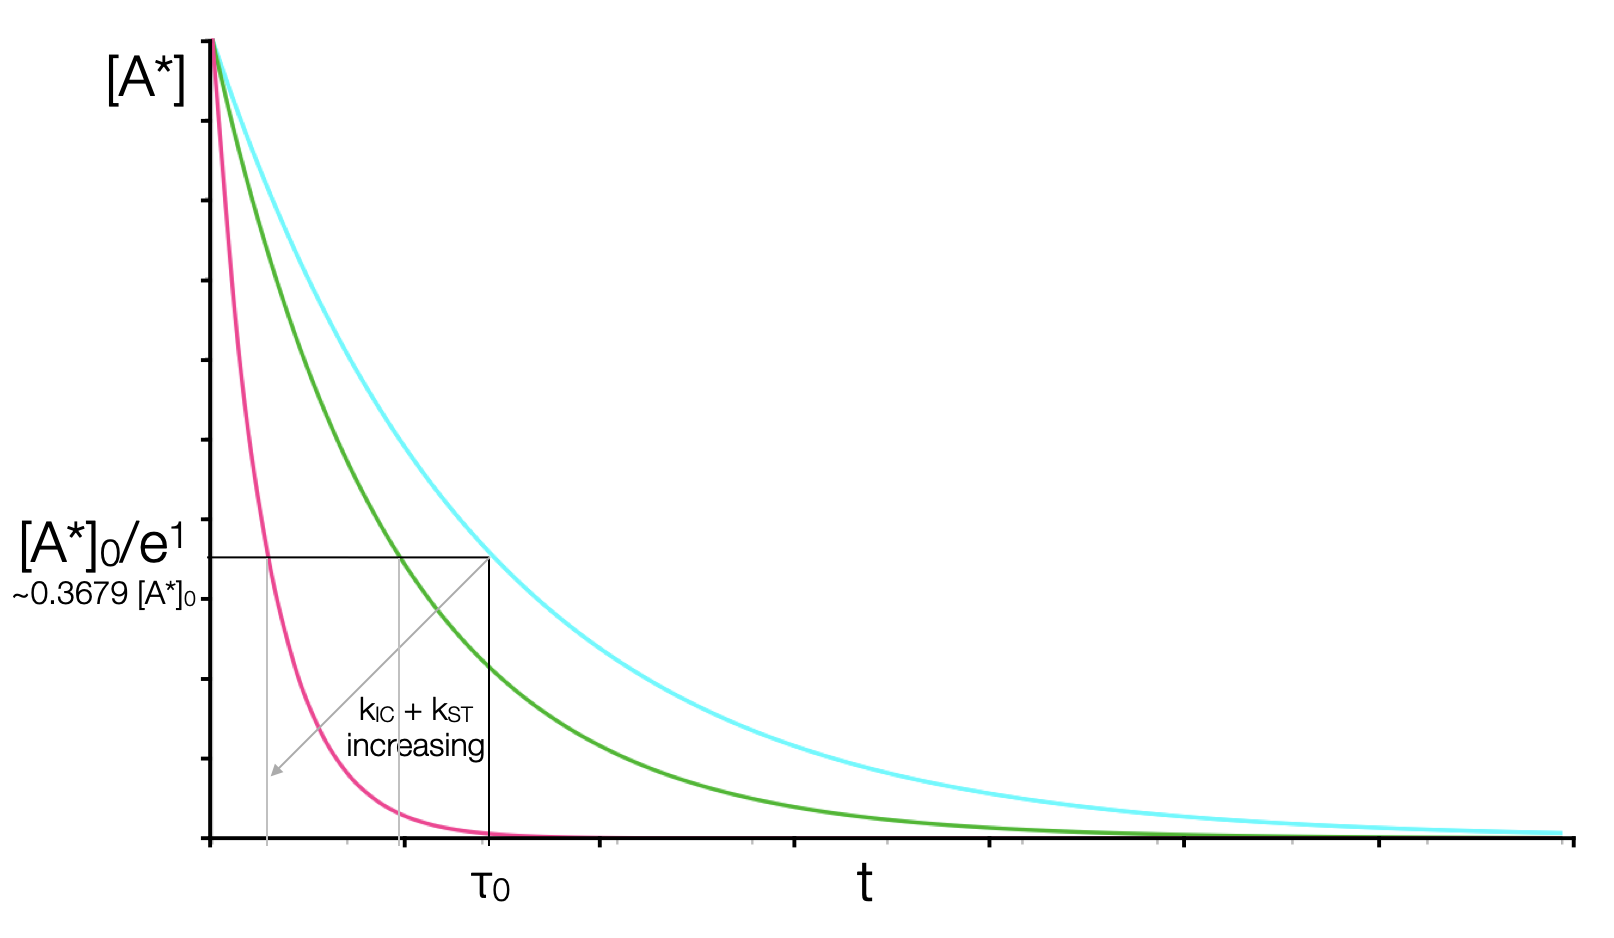
\includegraphics[width=0.7\linewidth]{images/rateslifetime} 

}

\caption{The variation of the emission lifetime (the time it takes to decay to 1/e of the initial concentration, for a constant rate of fluorescence emission but increasing rates of non-radiative decay.}\label{fig:rateslifetime}
\end{figure}

\hypertarget{sec:structure}{%
\section{Conceptual question - Effect of structure}\label{sec:structure}}

\emph{Fluorescein (figure \ref{fig:fluorescein}) in basic aqueous solution has a quantum yield of fluorescence, Φ\textsubscript{f}, of 0.95, and fluorescence lifetime, τ\textsubscript{f}, of 4.1 ns.}

\begin{figure}

{\centering 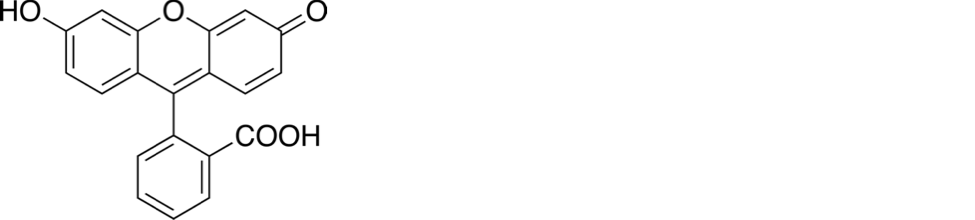
\includegraphics[width=0.7\linewidth]{images/fluorescein} 

}

\caption{The structure of the fluorescent molecule fluorescein}\label{fig:fluorescein}
\end{figure}

\emph{Suggest why the fluorescence quantum yield in this system is so high.}

The only things that affect the quantum yield and lifetime (equations \eqref{eq:lifetimefluor} and \eqref{eq:lifetimefluor}) are the different rate constants involved. The quantum yield is a measure of the proportion of excited states which decay by each pathway.

Therefore if the quantum yield of fluorescence is near unity then neither the rate of intersystem crossing or internal conversion is large. Intersystem crossing may occur due to the change in orbital type offered, but given the lack of heavy atoms this rate is unlikely to be high and will probably be a negligable proprortion given the high rates of other processes.

The rate of intersystem crossing is more efficient for rotations than vibrations (due to the closwer spacing of rotational energy levels), therefore if rotations can occur the rate of internal conversion tends to be quite high. In this case there is only one likely bond that could rotate to loose the excited state of the system. This is the single bond linking the two ring systems. Rotation around this bond is severly inhibited though due to the presence of the acid group which restricts rotation.

Please note that it is rotations around bonds that cross the conjugation within the molecule that allow for the most efficient energy loss.

\hypertarget{conceptual-question---lack-of-symmetry-in-spectra.}{%
\section{Conceptual question - lack of symmetry in spectra.}\label{conceptual-question---lack-of-symmetry-in-spectra.}}

\emph{The absorption and emission spectrum of fluorescein is shown in figure (\ref{fig:fluoresceinspec}).}

\begin{figure}

{\centering 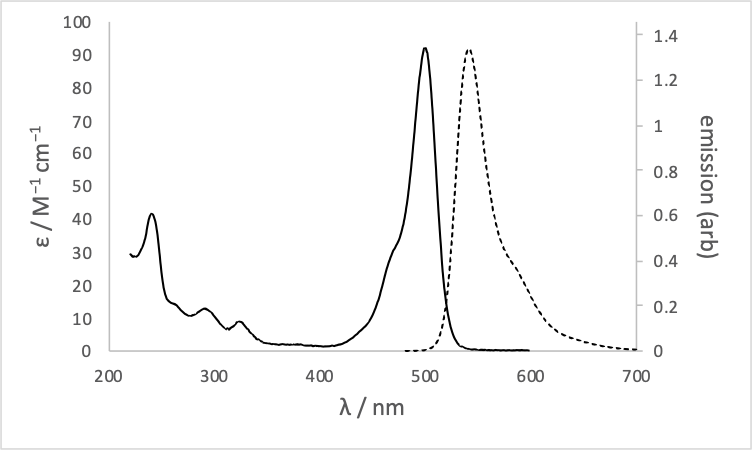
\includegraphics[width=0.7\linewidth]{images/fluoresceinspec} 

}

\caption{The absorption (solid) and emission (dashed) spectrum of fluorescein in basic ethanol.}\label{fig:fluoresceinspec}
\end{figure}

\emph{Why are the absorption bands between 200 -- 350 nm not reflected in the emission spectrum?}

Kasha's rule states \emph{"An excited state always emits from the lowest energy level of that spin multiplicity state.} Consequently we can excite into any available orbital, but the excited state will rapidly decay into the lowest energy level of that multiplicity. So although we are exciting from S\textsubscript{0} into S\textsubscript{1}, S\textsubscript{2}, S\textsubscript{3}\ldots{} any excited state will rapidly decay by internal conversion down to the S\textsubscript{1} excited state and all emission will occur from this state.

Kasha's rule is a consequence of the energy gap law which I alluded to when talking about the special case of azulene, but this will be covered in a video specifically talking about the energy gap law.

\hypertarget{sec:stokes}{%
\section{Conceptual question - Stokes' shift}\label{sec:stokes}}

\emph{The inorganic dye {[}Ru(bpy)\textsubscript{3}{]}\textsuperscript{2+} has a measured lifetime in water of 580 ns and a natural lifetime of 13.8 µs. The spectrum is shown in figure \ref{fig:Rubpyspec}. What is the origin of the large Stokes' shift in this system?}

\begin{figure}

{\centering 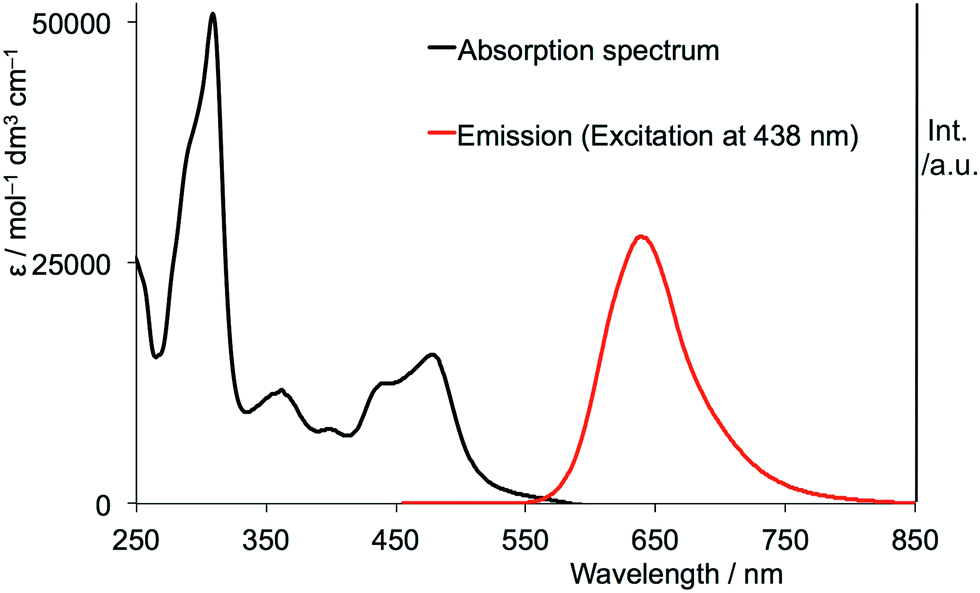
\includegraphics[width=0.7\linewidth]{images/Rubpy3spectra} 

}

\caption{The absorption (black) and emission (red) spectrum of ruthenium tris bypyridine in water.}\label{fig:Rubpyspec}
\end{figure}

Firstly we need to separate two things - the first is just the origin of the Stokes' shift due to the transition of an electron occuring very quickly leaving an optimised state to occupy an unoptimised state, which later relaxes. A typical Stokes' shift is \textasciitilde20 nm, the Stokes' shift in this example is more than 150 nm\ldots{} why?

If we consider the system that we have at hand, in this case {[}Ru(bpy)\textsubscript{3}{]}\textsuperscript{2+} we can note the HOMO-LUMO transition is an MLCT. This has a large difference in structure of the HOMO \& LUMO with a redistribution of charge which will also have a large effect on the arrangement of the solvent shell. Given this large difference in optimised structure there would be a large shift.

\begin{figure}

{\centering 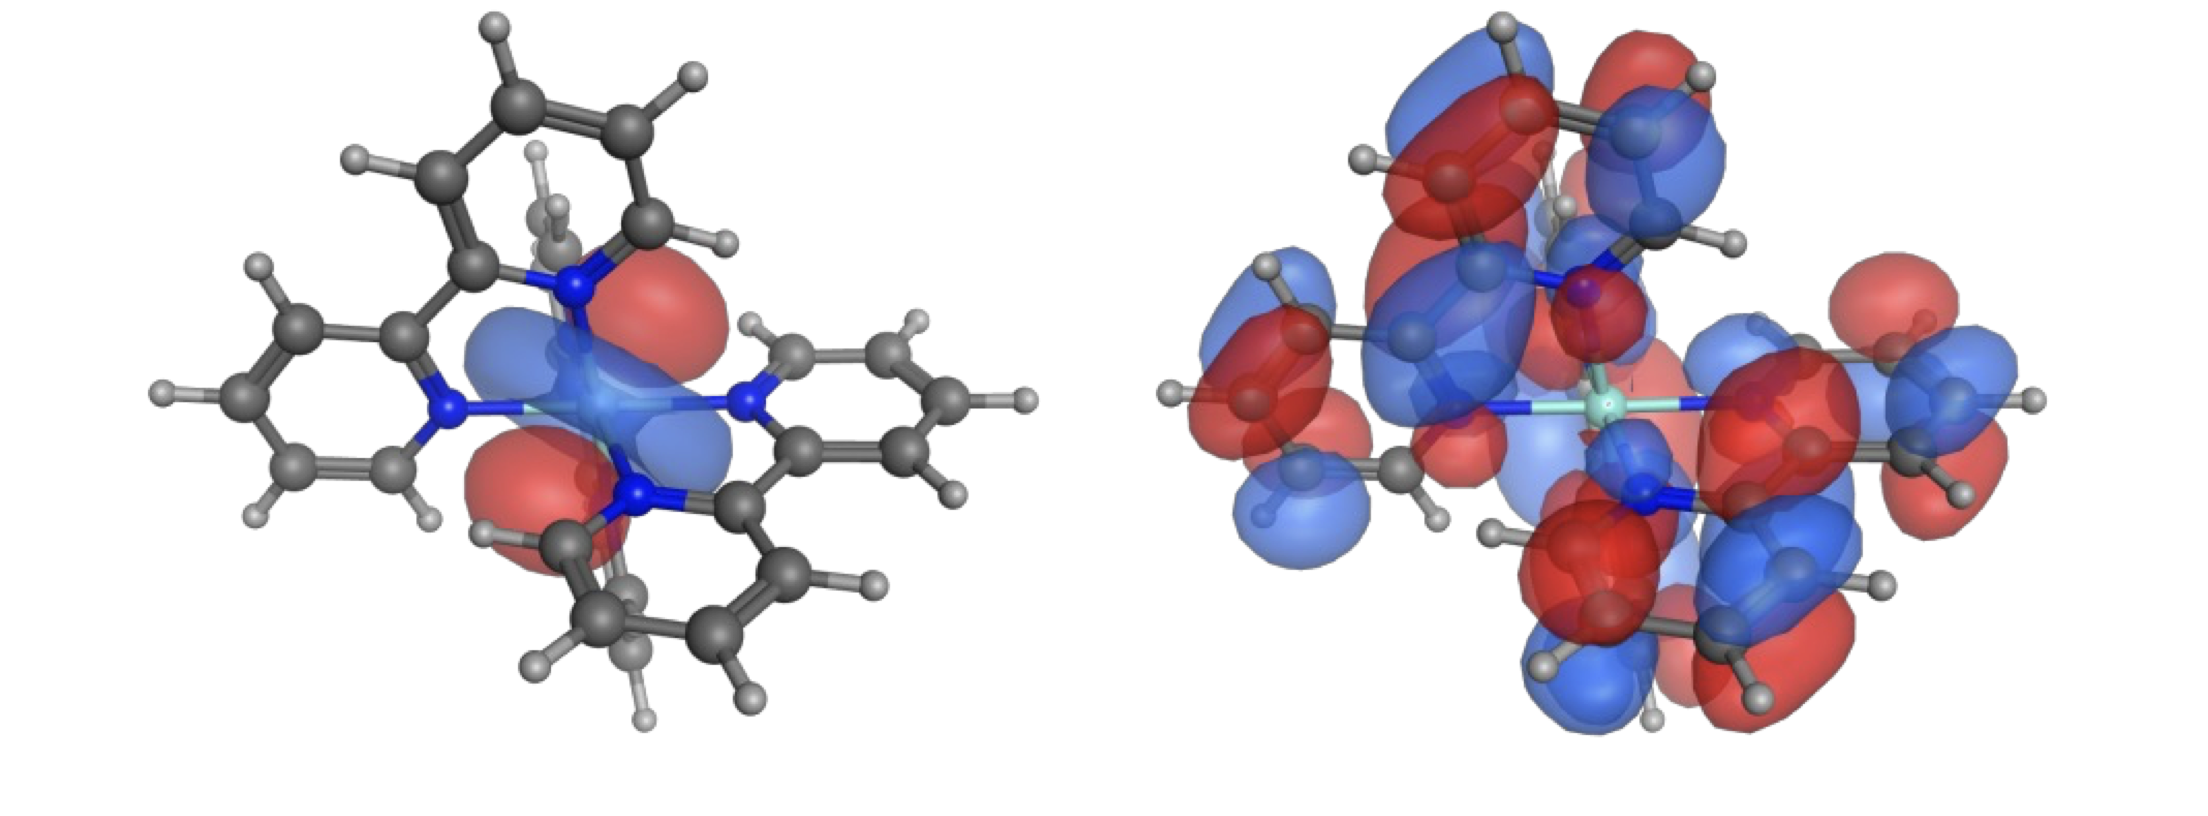
\includegraphics[width=0.7\linewidth]{images/RubpyMLCT} 

}

\caption{The HOMO (left) and LUMO (right) of ruthenium (II) tris bipyridine clearly showing the MLCT nature of the transition.}\label{fig:RubpyMLCT}
\end{figure}

However this isn't the only factor, the natural lifetime of 13.8 µs would indicate that the emission transition is phosphorescence, this spin forbidden transition has electrons alligned in parallel which is lower than the corresponding singlet state. So after excitation there is a change in multiplicity of the excited state, this lowers the energy of the system further moving the \(\lambda _{max}\) of emission to lower energy (longer wavelength).

Data from Shi \emph{et al.}, Synthesis and characterization of phosphorescent two coordinate copper(I) complexes bearing diamidocarbene ligands. \href{https://doi.org/10.1039/C6DT04016K}{Dalton Trans., 2017,46, 745-752.}

\hypertarget{sec:binding}{%
\section{Conceptual question - the effect of binding on emission}\label{sec:binding}}

\emph{The asymmetric cyanine dye YO-Pro-1 is a DNA stain because it has a large increase on fluorescence emission when binding to DNA. The lifetime in free solution is around 2 ps and when bound to DNA is 2.4 ns. What is the structural origin of the large increase of emission upon binding?}

\begin{figure}

{\centering 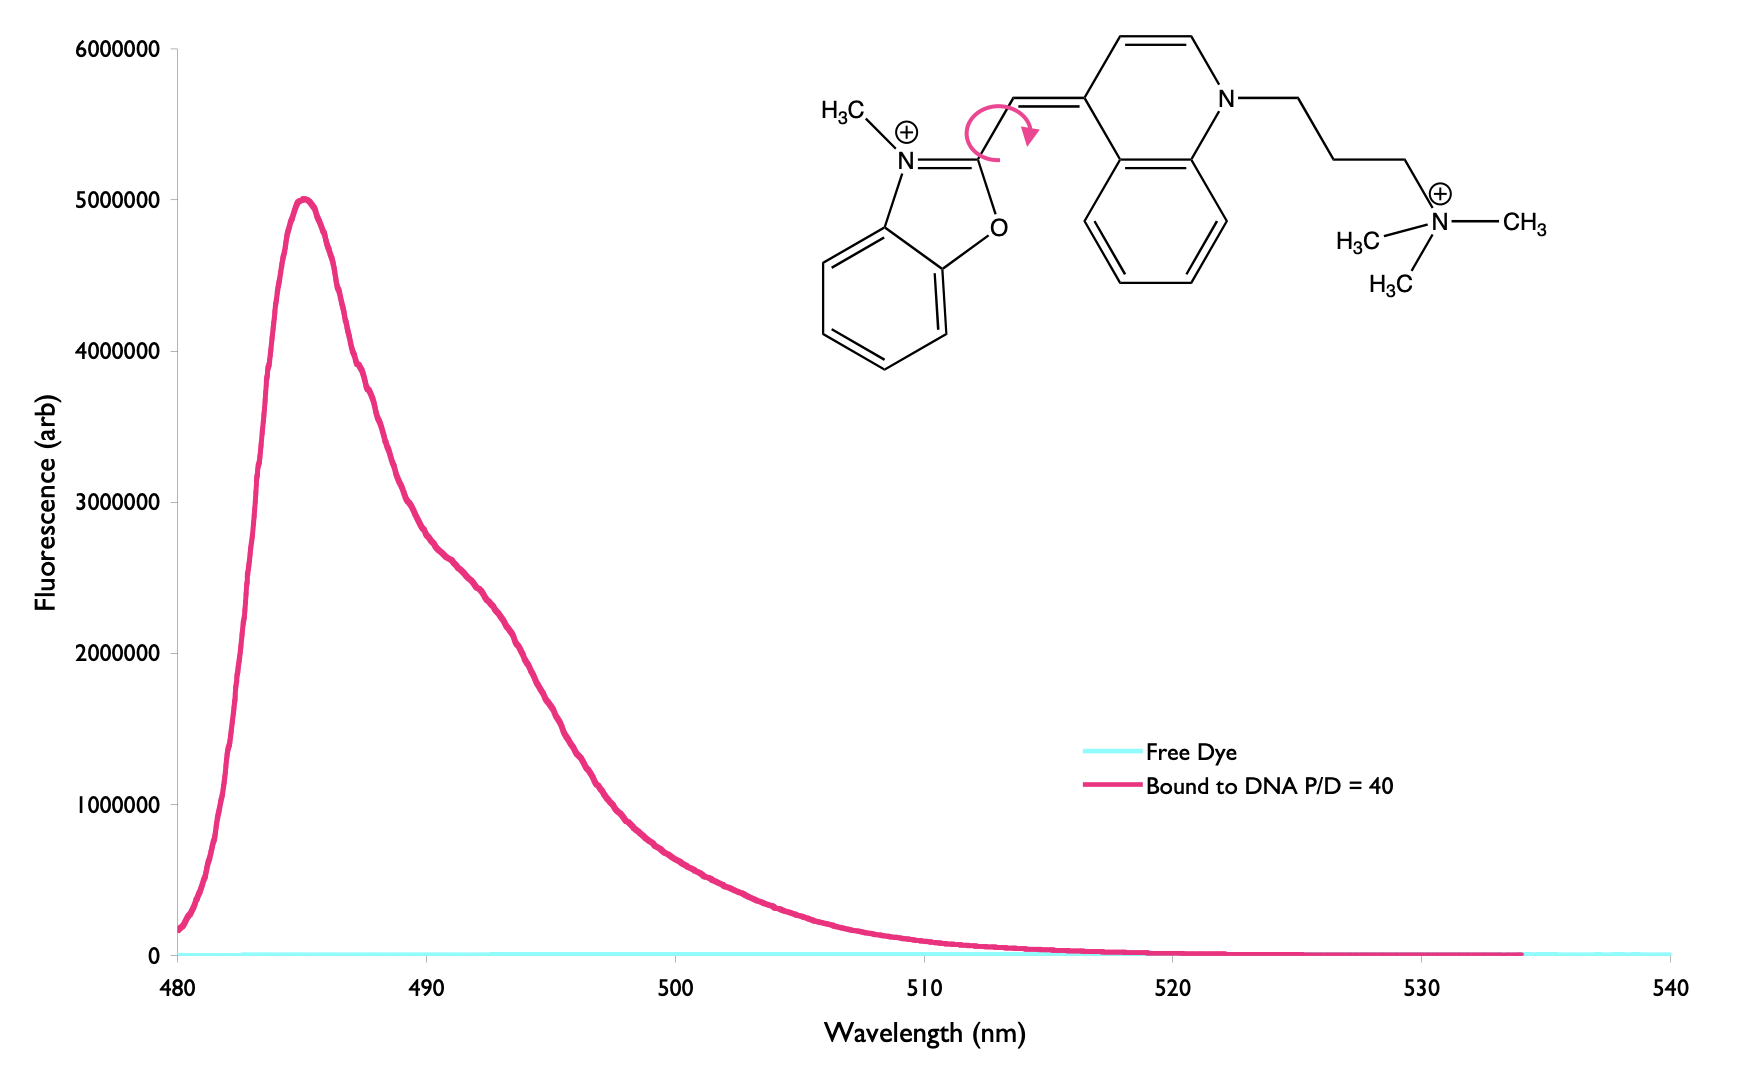
\includegraphics[width=0.7\linewidth]{images/YODNAans} 

}

\caption{The emission spectrum of the choromophore YO-Pro-1 when free in aqueous solution (blue) and when bound to DNA (pink), the structure of the chromophore indicating a route of rotation relaxation is indicated.}\label{fig:YODNA}
\end{figure}

The chromophore YO-Pro-1 has a methine bridge between the two halves of the chromophore, this offers efficient loss of the excited state \emph{via} internal conversion (see question \ref{sec:structure}. As noted earlier free rotation around a bond which cuts across the conjugation is particularly efficient in deactivating an excited state.

If this pathway is inhibited by binding to the DNA (the dye intercalates between the base pairs but any dye DNA interaction would inhibit this mechanism of excited state decay) then the fluorescence lifetime will increase (equation \eqref{eq:lifetimefluor}).

\hypertarget{extended-question---properties-of-ethidium-bromide-example-exam-question}{%
\section{Extended question - Properties of Ethidium Bromide (Example Exam Question)}\label{extended-question---properties-of-ethidium-bromide-example-exam-question}}

\emph{Ethidium bromide (EB, figure \ref{fig:ethidiumstructure} is used as a DNA stain, which is essentially non-fluorescent in aqueous solution, but shows a strong enhancement of emission upon binding to double stranded DNA (which has a negatively charged backbone).}

\emph{Emission is almost exclusively from the singlet excited state, but a triplet state has been shown to exist, which emits with a low quantum yield (Φ\textsubscript{P} = 0.00006).}

\begin{figure}

{\centering 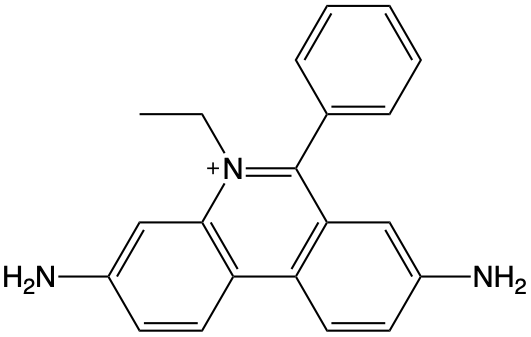
\includegraphics[width=0.3\linewidth]{images/ethidiumstructure} 

}

\caption{The structure of the cationic ethidium bromide chromophore.}\label{fig:ethidiumstructure}
\end{figure}

\emph{- Sketch a Jablonski diagram for the processes you know to occur.}

\begin{figure}

{\centering 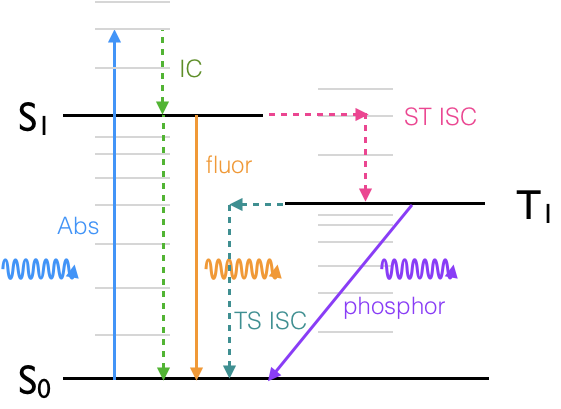
\includegraphics[width=0.6\linewidth]{images/Jablonski} 

}

\caption{A Jablonski diagram indicating the allowed transitions within the system, absorbance , internal conversion, intersystem crossing, fluorescence and phosphorescecne.}\label{fig:Jablonski}
\end{figure}

If phosphorescecne occurs there must be some intersystem crossing in both directions.

\emph{- The molar extinction coefficient, ε, of EB has be measured to be 78500 M\textsuperscript{−1} cm\textsuperscript{−1}. What factors contribute to EB having such a high extinction coefficient?}

There is a rigid structure indicating a similar ground and excited state strucutre, which would lead to a good overlap integrals between the HOMO and LUMO. THe molar extinction coefficient is a measure of this overlap integral.

\emph{The following spectra, lifetimes and quantum yield have been measured for EB in different free solution and DNA systems:}

Table: \label{tab:ethidiumlifetime} The lifetimes and quantum yields of ethidium bromide in aquous solution and when bound to DNA in protiated and deuterated systems.

\begin{longtable}[]{@{}lll@{}}
\toprule
& τ / ns & Φ\textsubscript{f}\tabularnewline
\midrule
\endhead
H\textsubscript{2}O (no DNA) & 1.6 & 0.012\tabularnewline
D\textsubscript{2}O (no DNA) & 6.3 &\tabularnewline
DNA & 28.3 & 0.220\tabularnewline
DNA (deuterated) & 38.4 &\tabularnewline
\bottomrule
\end{longtable}

\begin{figure}

{\centering 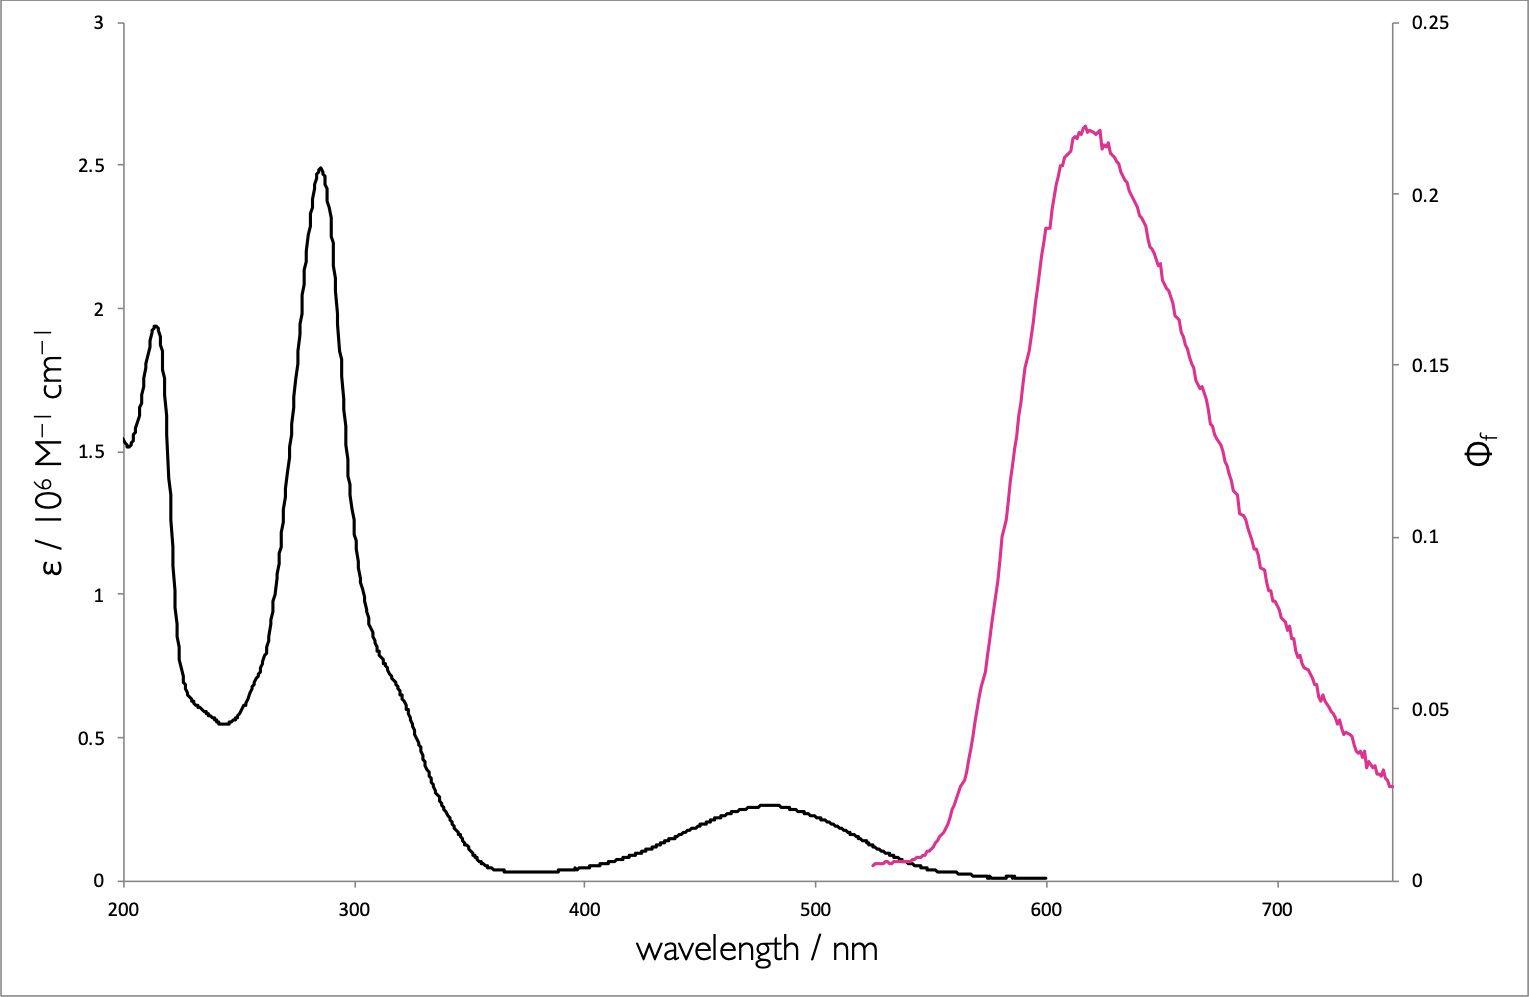
\includegraphics[width=0.7\linewidth]{images/ethidiumspectra} 

}

\caption{The absorption (black) and emission (pink) spectrum of ethidium bromide when bound to DNA.}\label{fig:ethidiumspectra}
\end{figure}

\emph{- What factors likely lead to an enhancement of fluorescence quantum yield upon binding to DNA?}

The chromophore single bond between the two halves of the chromophore, this offers efficient loss of the excited state \emph{via} internal conversion (see question \ref{sec:structure}. As noted earlier free rotation around a bond which cuts across the conjugation is particularly efficient in deactivating an excited state.

If this pathway is inhibited by binding to the DNA (the dye intercalates between the base pairs but any dye DNA interaction would inhibit this mechanism of excited state decay) then the fluorescence lifetime will increase (equation \eqref{eq:lifetimefluor}).

\emph{- Show that the natural lifetime of EB is 129 ns.}

\begin{equation*}
\phi_f = \frac{k_f^0}{k_f^0+k_{ic}+ k_{ST}+k_{\textrm{other}}}
\end{equation*}

\begin{equation*}
\tau_f = \frac{1}{k_f^0+k_{ic}+ k_{ST}+k_{\textrm{other}}}
\end{equation*}

The natural lifetime is the lifetime when the only decay pathway is fluorescence emission (equation \eqref{eq:natural}).

\begin{equation*}
\tau_f^0 = \frac{1}{k_f^0}
\end{equation*}

Combining equations \eqref{eq:lifetimefluor} and \eqref{eq:lifetimefluor}:

\begin{equation*}
\frac{\tau_f}{\phi_f}=\frac{\frac{1}{k_f^0+k_{ic}+ k_{ST}+k_{\textrm{other}}}}{\frac{k_f^0}{k_f^0+k_{ic}+ k_{ST}+k_{\textrm{other}}}}=\frac{1}{k_f^0}=\tau_f^0
\end{equation*}

Consequently \(\tau_f^0 = \frac{\tau_f}{\phi_f}=\frac{1.6}{0.012}= 129\) ns

\emph{- What is the origin of the large Stoke's shift (λ\textasciitilde max ex\textasciitilde{} = 520 nm, λ\textasciitilde max em\textasciitilde{} = 608 nm)}

We are told the transition is fluorescence, but it has a very long natural lifetime. This long lifetime would indicate that despite the transition being selection rule allowed there is a structural explanation for the inefficiency of this process.

This would indicate that there is now a poor overlap integral indcating a poor overlap of the excited state and ground state structures, or there is a large difference in the structures of the excited and ground states.

This large difference in structure would be accounted for in the Stokes' shift - a large deviation in structure would lead to a larger energy loss upon the optimisation of the excited state.

\emph{- What transitions are responsible for the absorption features in the:}
\emph{400-600 nm range
}200-350 nm range

The molecule has hetero atoms and so there will be both \(n-\pi*\) and \(\pi-\pi*\) transitions, the \(n-\pi*\) transitions will occur at lower energy (higher wavelength) and be the HOMO-LUMO transition.

\emph{- Why are the features in the 200-350 nm range not replicated in the emission spectrum?}

Kasha's rule states \emph{"An excited state always emits from the lowest energy level of that spin multiplicity state.} Consequently we can excite into any available orbital, but the excited state will rapidly decay into the lowest energy level of that multiplicity. So although we are exciting from S\textsubscript{0} into S\textsubscript{1}, S\textsubscript{2}, S\textsubscript{3}\ldots{} any excited state will rapidly decay by internal conversion down to the S\textsubscript{1} excited state and all emission will occur from this state.

\emph{- Why does deuterating the solvent (or DNA) effect the lifetime of the excited state?}

Ultimately because it affects the rates of internal conversion, and so the lifetime is changed as described in equation @\ref(eq:lifetimefluor). We will learn more as to why when we cover the energy gap law.

\emph{- What effect would freezing the samples have on the lifetime, fluorescence quantum yield \& phosphorescence quantum yield.}

You would expect the emission lifetime and quantum yield to increase on freezing (as described in equation @\ref(eq:lifetimefluor)) as the efficiency (and therefore rate) of internal conversion mechanisms (particularly rotational relaxation) would be dramatically reduced in solid systems.

\emph{A study of the thermodynamics of the dye DNA system measured the binding constant of EB with DNA to be 1.05 × 10\textsuperscript{6}.}

\emph{- Why is the measured quantum yield for a system containing 2 µM EB and 20 mM DNA only 0.18?}

This will be due to there being two states - one where the chromophore is bound, one where it is not. It is an equilibrium so not all dye will be bound to DNA. When not bound there is no fluorescence enhancement. The quantum yield we see is in fact a weighted average between the two states.

This is a problem solving question and any reasonable attempt would have been given credit. It is demonstrating an ability to think about data and the problem in a scientific manner.

\emph{- Why would increasing the ionic strength of the solution, increase the fluorescence intensity of EB in solution with DNA?}

This would push the equilibrium to form the dye:DNA complex increasing binding, as the binding increases the proportion of molecules displaying the higher quantum yield increases and the overall emission intensity of the sample increases.

This is a problem solving question and any reasonable attempt would have been given credit. It is demonstrating an ability to think about data and the problem in a scientific manner.

\hypertarget{ch:Workshop3}{%
\chapter{Workshop Questions for Week 3}\label{ch:Workshop3}}

\hypertarget{sec:overlap}{%
\section{Short conceptual question - Electronic-vibrational overlap integrals}\label{sec:overlap}}

\begin{figure}

{\centering 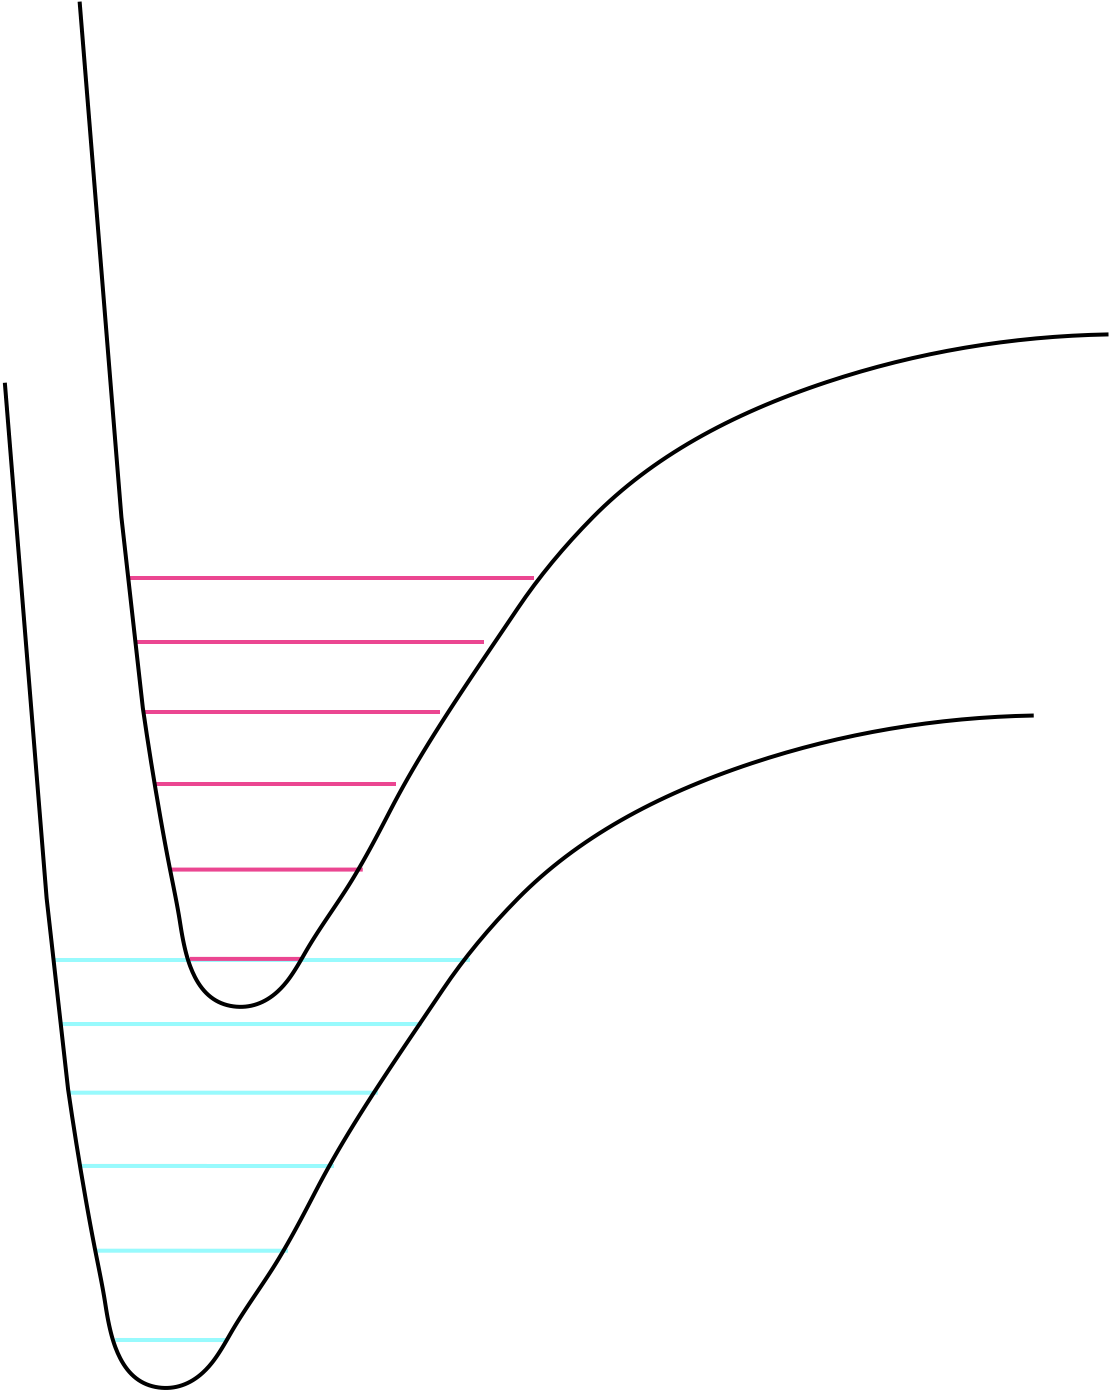
\includegraphics[width=0.3\linewidth]{images/overlap} 

}

\caption{The grond and excited state potential wells and the vibrational levels within them.}\label{fig:overlap}
\end{figure}

\emph{On the figure sketch the vibrational energy levels in the ground and the excited state.}

\emph{How would the following affect this overlap integral?}

\begin{enumerate}
\def\labelenumi{\arabic{enumi}.}
\item
  \emph{Energy gap.}
\item
  \emph{The vibrational energy gaps}
\item
  \emph{Reaction coordinate (the difference in structure between ground and excited state)}
\end{enumerate}

\begin{figure}

{\centering 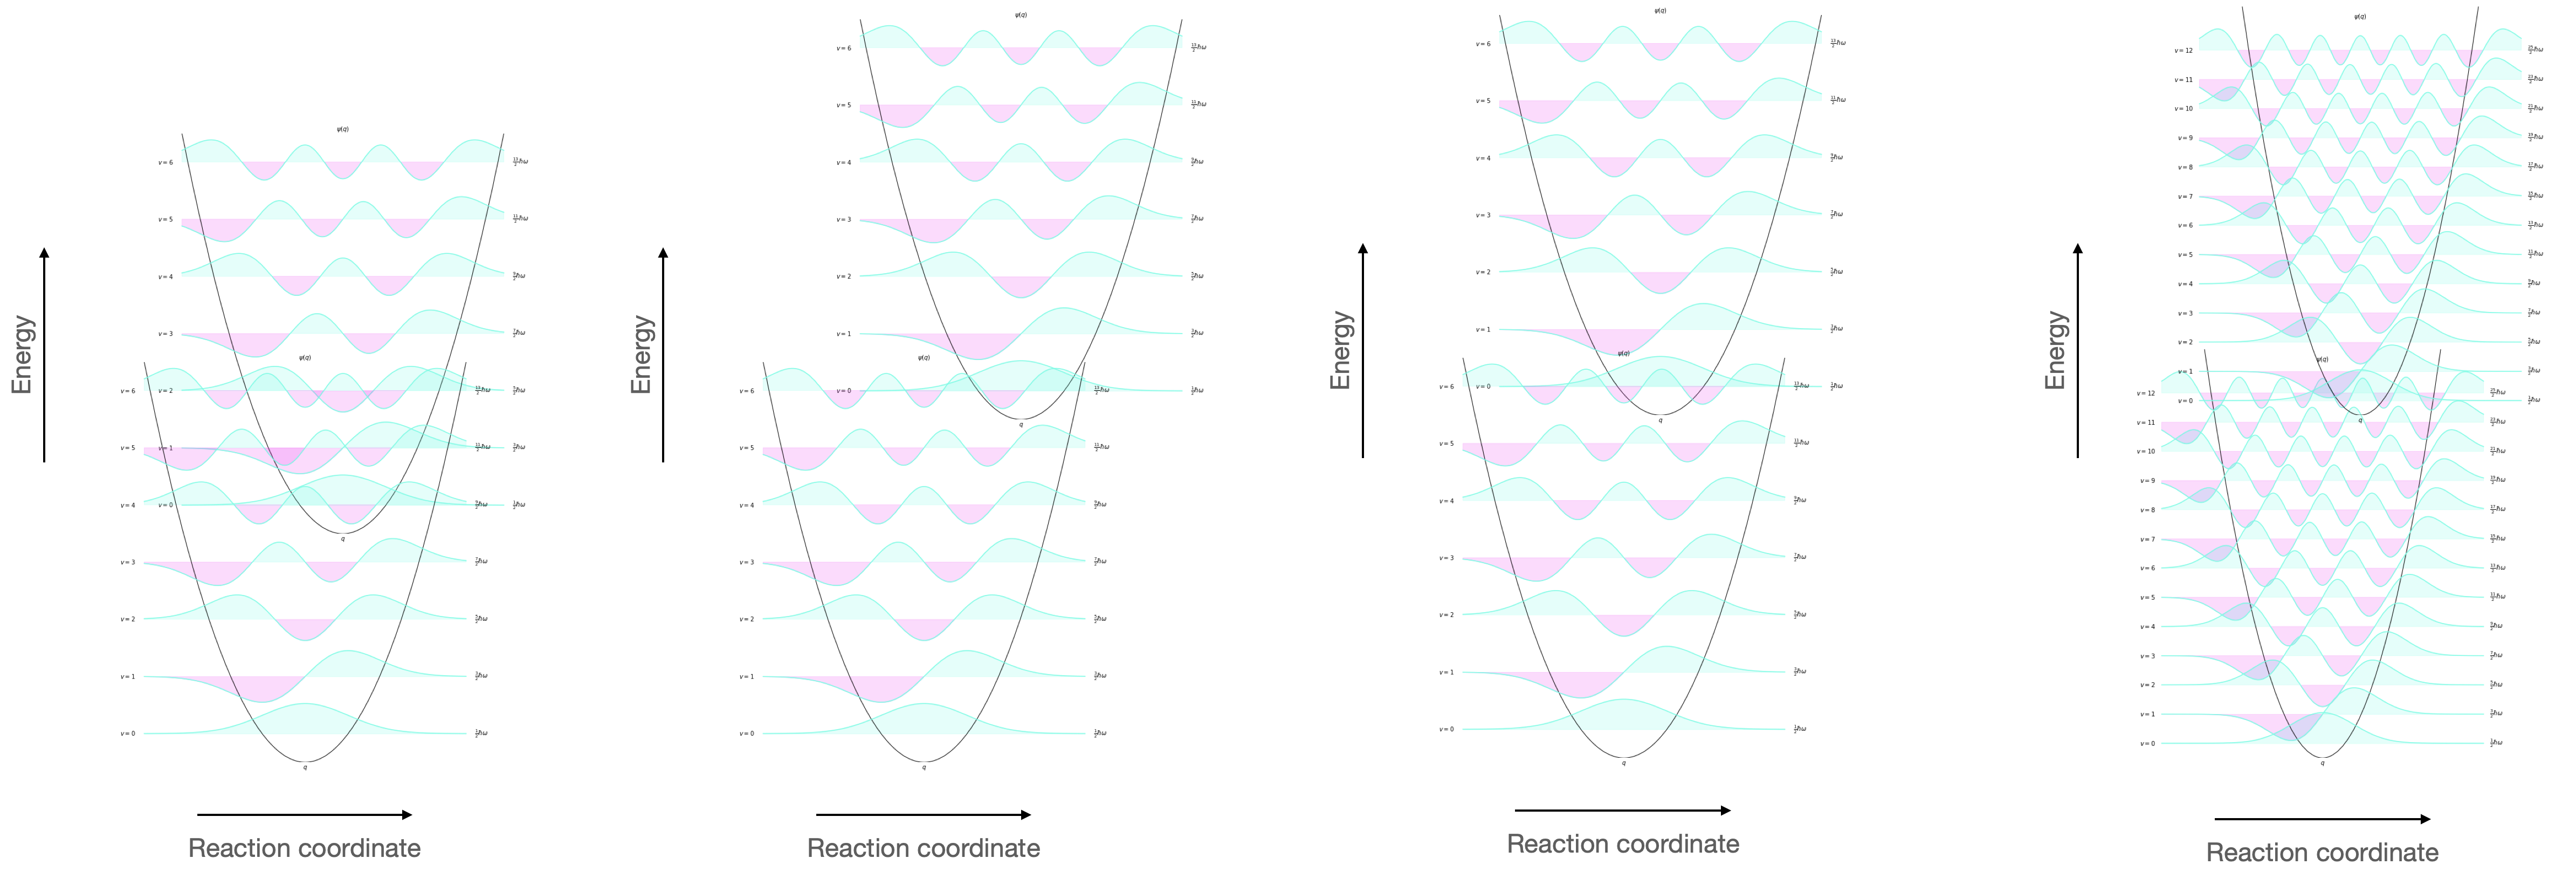
\includegraphics[width=1\linewidth]{images/intconvoverlap2} 

}

\caption{The vibrational wavefunctions of the HOMO and LUMO showing the overlap (visualised as the overlapping of the wavefunctions). This overlap integral depends upon (left) the energy gap of HOMO and LUMO, the reaction coordinate (second left) and the spacing of vibrational energy levels (right).}\label{fig:overlapans}
\end{figure}

In each case the overlap integral between the HOMO and LUMO is different, and therefore the associated rate of internal conversion will be different.

Remember that the rate of internal conversion to the lowest vibrational level in any electronic excited state is high, and so we are looking at the overlap between the v' = 0 and v = n states.

\hypertarget{sec:structureQY}{%
\section{Short conceptual question - The effect of structural changes on quantum yield}\label{sec:structureQY}}

\emph{5,10-dihydroindeno{[}2,1-a{]}indene and trans-stilbene (figure \ref{fig:stilbeneindene}) are similar in structure but have very different fluorescent quantum yields of 1.00 and 0.05 respectively, however for trans-stilbene this increases to 0.75 at 77 K. Suggest a reason for the difference in quantum yield of:}

\begin{itemize}
\tightlist
\item
  \emph{the two molecules}
\item
  \emph{the two temperatures}
\end{itemize}

\begin{figure}

{\centering 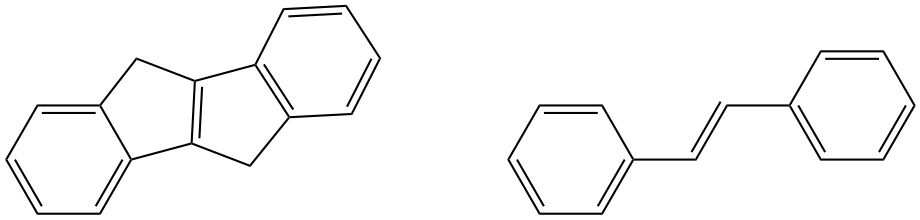
\includegraphics[width=0.6\linewidth]{Images/stilbeneindene} 

}

\caption{5,10-dihydroindeno[2,1-a]indene (left) and trans-stilbene (right)}\label{fig:stilbeneindene}
\end{figure}

If we consider the difference in quantum yield of the two chromophores then rotational pathways aren't available to the indine choromophore.

Considering this on a more mathematical level (but still with no maths), for the stilbene there is a large difference in the ground and excited state structures (because the excited state reduces the bond order of the highest energy bond (the non aromatic π bond) giving these atoms sp\textsuperscript{3} character).

This would indicate that the two potential wells are offset by a larger amount leading to a good overlap integral between the HOMO and LUMO states which is not available when the difference in reaction coordinate is smaller.

However the structure of the indine in ground and excited state is similar and so the overlap integrals will be much smaller.

When considering the effect of temperature on the quantum yield of stilbene, at first you may consider this to not have an effect (as there is no temperature term in the energy gap law), however, there is now no longer free rotation allowed and so the closely spaced rotational levles (which allow very efficient excited state deactivation) are no longer the principle deactivation pathway.

\hypertarget{sec:ratephos}{%
\section{Short mathematical question - Effect of the rate of singlet triplet intersystem crossing on th quantum yield of phosphorescence}\label{sec:ratephos}}

\emph{Why is it likely that the quantum yield of phosphorescence of a sample would increase after the sample is frozen.}

The quantum yield of phosphorescence (\(\phi_p\))depends upon the quantum yield of singlet to triplet intersystem crossing (\(\phi_{ST}\)), as described in equation \eqref{eq:QYphos}.

\begin{equation}
\phi_p = \phi_{ST}\frac{k_p^0}{k_p^0+ k_{TS}+k_{\textrm{other}}}
\label{eq:QYphos}
\end{equation}

with the quantum yield of singlet to triplet intersystem crossing (\(\phi_{ST}\)) given by equation \eqref{eq:QYST}

\begin{equation}
\phi_{ST} = \frac{k_{ST}}{k_f^0+k_{ic}+ k_{ST}+k_{\textrm{other}}}
\label{eq:QYST}
\end{equation}

So as with Question \ref{sec:structureQY} we have the reduction of reate of internal conversion (\(k_{IC}\)) falls when the sample is frozen as the rotational deactivation pathways are no longer available. If \(k_{IC}\) is smaller (and other rates don't change), then the quantum yield of singlet to triplet intersystem crossing (\(\phi_{ST}\)) increases.

\hypertarget{sec:calcphos}{%
\section{Short mathematical question - Determining the quantum yield of phosphorescence}\label{sec:calcphos}}

\emph{A molecule decays by a combination of internal conversion, intersystem crossing and phosphorescence. What is the quantum yield of phosphorescence?}

\begin{itemize}
\tightlist
\item
  k\textsubscript{IC} = 2.1 × 10\textsuperscript{11} s\textsuperscript{−1}
\item
  k\textsubscript{ST} = 2.9 × 10\textsuperscript{9} s\textsuperscript{−1}
\item
  k\textsubscript{TS} = 7.4 × 10\textsuperscript{6} s\textsuperscript{−1}
\item
  k\textsubscript{p}\textsuperscript{o} = 6.2 × 10\textsuperscript{8} s\textsuperscript{−1}
\end{itemize}

Using equations \eqref{eq:QYST} \& \eqref{eq:QYphos} we can see (\(k_f^0=0\)):

\begin{equation*}
\phi_{ST} = \frac{2.9 × 10^9}{2.1 × 10^{11}+2.9 × 10^9}
\end{equation*}

and

\begin{equation*}
\phi_p = \left(\frac{2.9 × 10^9}{2.1 × 10^{11}+2.9 × 10^9}\right)\left(\frac{6.2 × 10^8}{6.2 × 10^8+ 7.4 × 10^6}\right)
\end{equation*}

\(\phi_p=0.013\)

This value is really very small, driven principally by the high efficiency of the internal conversion from the singlet state.

\hypertarget{sec:exhydrocarbons}{%
\section{Short conceptual question - Deactivation of excited state aromatic hydrocarbsons}\label{sec:exhydrocarbons}}

\begin{longtable}[]{@{}llll@{}}
\caption{\label{tab:smallmolQY} The quantum yields of various deactivation processes in small organic molecules measured at 77 K in a glass matrix.}\tabularnewline
\toprule
& Φ\textsubscript{f} & Φ\textsubscript{ST} & ΔE / kJ mol\textsuperscript{−1}\tabularnewline
\midrule
\endfirsthead
\toprule
& Φ\textsubscript{f} & Φ\textsubscript{ST} & ΔE / kJ mol\textsuperscript{−1}\tabularnewline
\midrule
\endhead
Napthalene & 0.20 & 0.80 & 385\tabularnewline
Anthracene & 0.70 & 0.30 & 318\tabularnewline
Pyrene & 0.6 & low & 322\tabularnewline
Tetracene & 0.1 & 0.65 & 251\tabularnewline
Pentacene & 0.10 & 0.15 & 209\tabularnewline
\bottomrule
\end{longtable}

\emph{When examining the data above suggest why it is likely why the quantum yields of both fluorescence and singlet to triplet intersystem crossing decrease with increasing molecule size.}

Firstly I've listed the quantum yield of two decay pathways but we have to elucidate (or estimate) the quantum yield of internal conversion by deduct the listed quantum yield values from unity (the probability of all decay pathways from a given state has to be 1).

There are two important factors at play here, the rigid structure (in both ground and excited state) of the chromophores and the HOMO-LUMO energy gap.

If I start by considering napthalene this molecule has a large HOMO-LUMO energy gap and so we would expect there to be only a small overlap of the wavefunctions between the ground and excited state for efficient transitions of an electron from the excited state to ground state potential well.

As this energy gap becomes smaller you would expect there to be a relative increase in rate of the internal conversion pathway as the overlap integral gets bigger. This is particularly true for rigid structures where at high vibrational level of the ground state (and small difference in reaction coordinate) you expect a better overlap integral as ΔE becomes smaller (see figure \ref{fig:overlapans}).

So if the rate of internal conversion increases, then the quantum yields of both singlet to triplet intersystem crossing and fluorescence will decrease.

\hypertarget{sec:dsolvent}{%
\section{Short conceptual question - Affect of deuteration of solvents.}\label{sec:dsolvent}}

\emph{Singlet oxygen has a phosphorescence wavelength of around 1070 nm and a lifetime of 2 µs in water, how would you expect this lifetime to change for singlet oxygen in D\textsubscript{2}O?}

This question is here to show that internal conversion by coupling to the solvent works in much the same way as internal conversion within a molecule.

Excited states of chromophores in the gas phase have a longer lifetime than any solution based systems.

\hypertarget{sec:isotope}{%
\section{Short conceptual question - Isotope effects on deactivation of an excited state}\label{sec:isotope}}

The fluorescence quantum yield and singlet state lifetime of both proteated and deuterated pyrene are 0.90 and 450 ns respectively. Why does deuteration of the sample have no measureable affect on these values?

Conversely for naphthalene phosphorescence (in glass at 77 K) the quantum yield of phosphoresce increases from 0.05 to \textasciitilde0.80 on deuteration of the sample. (ΔE = 251 kJ mol\textsuperscript{−1} ). Explain this observation with respect to the energy gap law.

\emph{(This will be a discussion question - please feel free to raise a hand or write comments in the zoom chat)}

\hypertarget{sec:heavy}{%
\section{Short conceptual question - The effect of heavy attoms on the rate of intersystem crossing}\label{sec:heavy}}

\begin{longtable}[]{@{}llll@{}}
\caption{\label{tab:heavyatom} The affect of substitution of different halogens on the rates of phosphorescence and singlet to triplet intersystem crossing.}\tabularnewline
\toprule
& k\textsubscript{p} & k\textsubscript{ST} & Φ\textsubscript{p} / Φ \textsubscript{f}\tabularnewline
\midrule
\endfirsthead
\toprule
& k\textsubscript{p} & k\textsubscript{ST} & Φ\textsubscript{p} / Φ \textsubscript{f}\tabularnewline
\midrule
\endhead
Napthalene & 0.05 & 0.39 & 0.09\tabularnewline
1-fluoronaphthalene & 0.23 & 0.42 & 0.07\tabularnewline
1-chloronaphthalene & 1.1 & 2.35 & 5.2\tabularnewline
1-bromonaphthalene & 13.5 & 36.5 & 169\tabularnewline
1-iodonaphthalene & 190 & 310 & \textgreater760\tabularnewline
\bottomrule
\end{longtable}

Briefly explain why the rates of these processes increase as we move down the group.

\emph{(This will be a discussion question - please feel free to raise a hand or write comments in the zoom chat)}

\hypertarget{sec:osphen}{%
\section{Short conceptual question - The effect of absorbance and emission wavelengths on the quantum yield of emission}\label{sec:osphen}}

\begin{longtable}[]{@{}llllll@{}}
\caption{\label{tab:osphen} The spectroscopic details of a family of osmium complexes.}\tabularnewline
\toprule
& λ\textsubscript{abs} / nm & λ\textsubscript{em} / nm & ΔE / eV & τ/ ns & Φ\textsubscript{em}\tabularnewline
\midrule
\endfirsthead
\toprule
& λ\textsubscript{abs} / nm & λ\textsubscript{em} / nm & ΔE / eV & τ/ ns & Φ\textsubscript{em}\tabularnewline
\midrule
\endhead
{[}Os(phen)\textsubscript{3}{]}\textsuperscript{2+} & 650 & 720 & 0.186 & 260 & 0.016\tabularnewline
{[}Os(phen)\textsubscript{2}(dppene){]}\textsuperscript{2+} & 455 & 609 & 0.69 & 1830 & 0.138\tabularnewline
{[}Os(phen)(dppene)\textsubscript{2}{]}\textsuperscript{2+} & 400 & 530 & 0.761 & 3600 & 0.518\tabularnewline
\bottomrule
\end{longtable}

Why does the fluorescence lifetime increase as the phenanthroline ligands are replaced with dppene ligands?

\emph{(This will be a discussion question - please feel free to raise a hand or write comments in the zoom chat)}

  \bibliography{book.bib,packages.bib}

\end{document}
